\documentclass{article}

\usepackage[utf8]{inputenc}
\usepackage{mathtools, amssymb}
\usepackage{caption}
\usepackage{subcaption}
\usepackage{graphicx}
\usepackage{booktabs}

\graphicspath{ {./images/} }

\DeclarePairedDelimiter{\abs}{\lvert}{\rvert}
\DeclarePairedDelimiter{\norm}{\lVert}{\rVert}

\newcommand*\mean[1]{\bar{#1}}

\title{Learn to Scale}
\author{alex.kreimer, ilan.shimshoni}
\date{May 2016}

\begin{document}

\maketitle

\begin{abstract}
  The size of a translation vector for a single moving camera is not
  directly observable, although is desirable.  Stereo, scene/camera
  prior assumptions were used in the past to recover the translation
  size.  We argue that the required information is present in the
  images and explore a number of ways to learn it.  We experiment with
  both ``legacy'' shallow learning methods and hand-crafted features
  as well as end-to-end learning methods based on the convolutional
  neural networks.
\end{abstract}

\section{Introduction}

Recovering camera 6-DOF ego-motion from images is a well studied
problem. It arises in various practical contexts
(e.g. virtual/augmented reality application, autonomous or aided
navigation, etc.).  The problem was studied in both stereo and the
monocular setups.  To recover the full 6-DOF motion, the previous
works resorted to the stereo setup, used auxiliary sensors (e.g. IMU)
or made assumptions about the camera pose and the scene.  All of these
have their drawbacks: stereo pairs are fragile and require careful
calibration procedures, additional sensors are not always available
and also require calibration, scene assumptions don't always hold.
Motion estimation from images of a single moving camera is probably
the hardest setup, as well as the most desirable one, because of its
simplicity.  It is well known that the translation scale parameter is
not directly observable for a motion of a single camera.

We argue, that for natural scenes the scale information is present in
the images and may be extracted.  Our method learns a regressor, that
is capable to prediction the motion scale.

\section{Related work}

\subsection{Others}
\subsection{Our method}

We assume that a single camera moves through space and takes images.
We treat the initial camera pose (at time $t=0$) as the world
coordinate frame.  We denote the pose of the camera at time $t$ by
$\mathbf{\hat{T}}_t$ described by the rotation matrix
$\mathbf{\hat{R}}_t$ and the translation vector $\mathbf{\hat{t}}_t$
as seen in the world coordinate frame.  We denote camera image taken
at time $t$ by $I_t$.  To facilitate the discussion, we also introduce
notation for camera pose
$\mathbf{T}_t = [\mathbf{R}_t\ |\ \mathbf{t}_t] $ as seen from the
coordinate frame associated with camera pose at time $t-1$.  Most of
the time, we will omit the time index, since its clear from the
context.  By translation scale (or simply, scale) we refer to the norm
of the translation vector $\mathbf{t}$ (e.g.,
$s = \lVert \mathbf{t} \rVert$)

We pose the scale estimation problem as a regression problem and
search for a good regressor model.

\section{Random forest}

\subsection{Decision trees}

In this section we briefly describe tree-based methods for regression.
These involve splitting the feature space into a number of small
regions.  The prediction for a sample is made by computing a mean or a
mode of training samples that belong to the same region.  Since the
set of rules used to split the feature space into smaller regions may
be described by a tree, these methods are referred to as
\textit{decision tree} methods.

Building a decision tree may be described by a two step procedure:
\begin{enumerate}
\item Split the feature space, e.g., the set of all possible values
  for $X_1, X_2,\ldots,X_n$ into $J$ distinct regions $R_1, R_2,\ldots, R_J$.
\item For every sample that belongs to the regions $R_i$ we make the
  same prediction, which is a mean of the responses of training
  samples that belong to this region.
\end{enumerate}

The regions $R_i$ are usually chosen to be multidimentional boxes (axis aligned).  We would like to find such a partition of the feature space that minimizes
\begin{equation}\label{eq:tree_objective}
\sum\limits_{j=1}^J\sum_{x\in R_j}{(x-\mean{x}_j)^2}
\end{equation}

Where $\mean{x}_j$ denotes the mean of the response values of the
samples in region $R_j$.  Unfortunately, solving the optimization
problem~\ref{eq:tree_objective} is computationally hard.  Usually it
is replaced with a greedy algorithm, called \textit{recursive binary
  splitting}.  This approach starts at the top of the tree and
greedily chooses the best split at that point that minimizes the
variance of its subtrees.  To be more precise, for each $j$ and $s$ we
define the hyperplanes:

\begin{equation}
  R_1(j,s) = \{ X\lvert X_j<s \}\quad\text{and}\quad R_2(j,s) = \{ X\lvert X_j \geq s \},
\end{equation}

We seek such $j$ and $s$ that minimize the equation:

\begin{equation}
  \sum\limits_{i:x_i\in R_1(j,s)}{(y_i-\hat{y}_{R_1})}^2 + \sum\limits_{i:x_i\in R_2(j,s)}{(y_i-\hat{y}_{R_2})}^2,
\end{equation}

Where $y_{R_1}, y_{R_2}$ are the averate responses of the samples in
$R_1(j,s), R_2(j,s)$ respectively.  Once we found the $j$ and $s$ we
recursively split each subtree in a similar manner.  The process is
repeated until stopping criterion (e.g., number of nodes in the leaf)
is reached.

\subsection{Bagging}
The decision trees tend to suffer from \textit{high variance}. This
means that if we split the training set into a number of random
subsets and fit random tree into each subsample, we would likely to
get much different answers from these trees when asked the same
question.  It is known that the variance of a mean of a set of
independent random variables is $\frac{1}{n}$.  Thus, in order to
improve the variance of the estimator, it is possible to fit $n$
estimators, each to its training-set and the average their
predictions.  Since, usually, we don't have $n$ training sets, we
would use \textit{bootstrapping} (e.g., sample independently with
replacement from the data set).

\subsection{Random Forest}
Random forest suggest additional improvement over bagging, by
decorrelating the random trees.  The issue they attempt to address is
this: lets say there is a very dominant feature w.r.t. to task at hand
for a given dataset.  Bagging ensures that we use different training
sets, but yet, most trees will tend to first split on this dominant
feature.  In this case the trees will resemble each other.  In random
forest, the trees are constructed by using only a subset of features
(e.g., $m = \sqrt{p}$).  This means that at calculating the splits,
the algorithm is allowed to consider only a subset of features.

\section{Convolutional Neural Networks}

Convolutional neural networks (CNN) leverage the availability of the
computational power and the abundance of data.  CNNs have become a
method of choice in a number of computer vision areas (e.g., image
classification, object recognition).  They were also shown capable of
per-pixel tasks, such as semantic segmentation and depth estimation
from a single image. Works like (e.g., flownet) show that CNN's can do
well for task that require feature matching as well as feature
extraction.

With these encouraging works in mind, we turn to CNN for our task.
There are lots of network architectures out there to choose from. We
have decided to use the ZF object recognition network as a basic
building block for our work.

\begin{figure}[h!]
  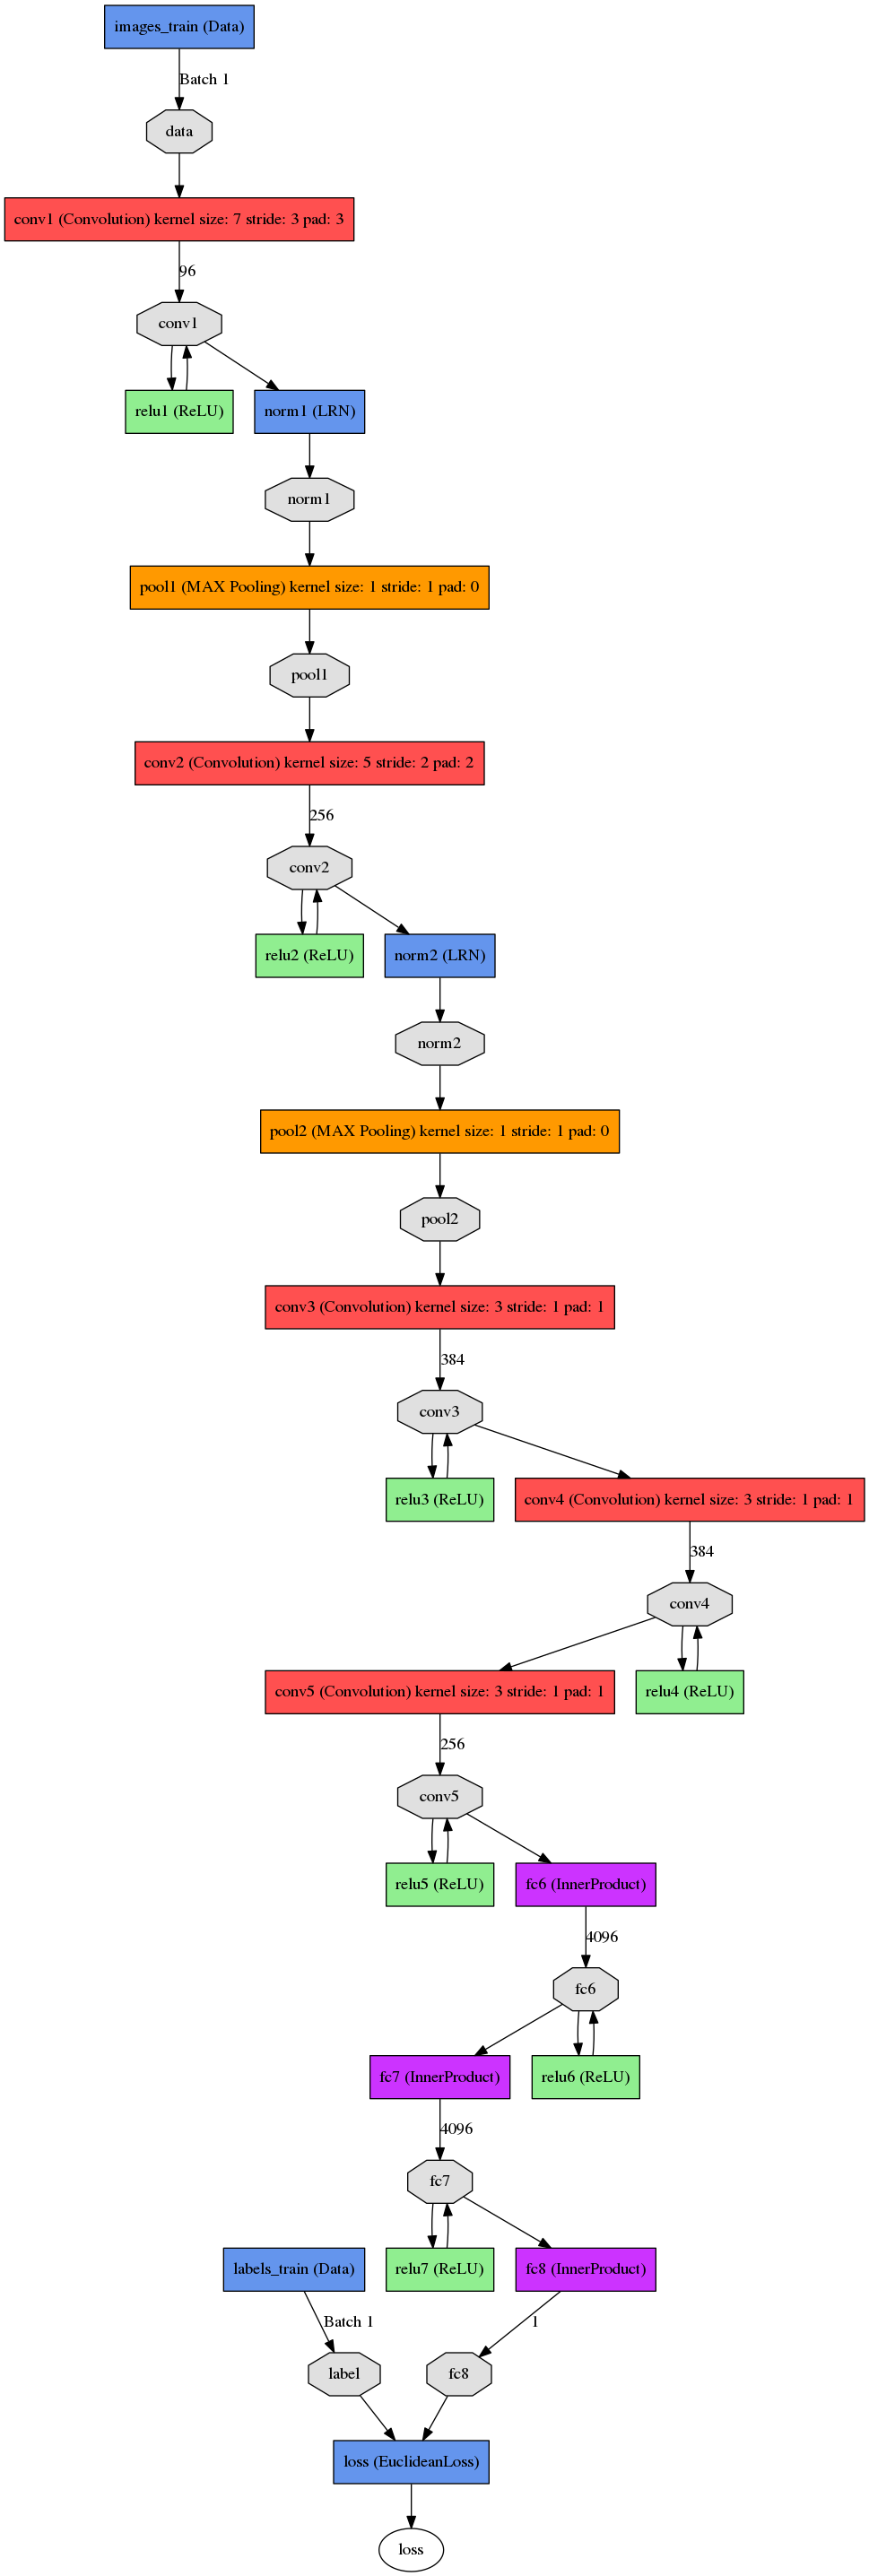
\includegraphics[width=0.9\linewidth]{ZF}
  \caption{Example image of the extracted corners}
  \label{fig:ex_corners}
\end{figure}

\section{LSTM}

\section{Experiments}

\subsection{Random Forest}
The feature vectors are created as follows: we extract and match
sparse salient points in both input images.  The output of this stage
is a set of a corresponding pixel locations.  Then, we compute the
point displacement magnitudes.  Finally, we bin all the interest
pundits according to a grid and create histogram of displacement
magnitudes for each bin.  Concatenating all histograms together
produces a feature vector.  Salient point choice, point matching
method, grid and histogram size are the parameters of the algorithm we
experiment with.

\subsection{Corner Extraction and Matching}

\emph{Note:} by corners we mean the image corners and by features we
denote the machine learning features.

We use Harris corners and square $11\times 11$ patches as corner
descriptors. SSD is used as a distance measure with the winning pair
declared a match.  To prune the outliers we fit the fundamental into
the matched corner sets and remove the corners that do not agree with
this model.  See Figure~\ref{fig:ex_corner_and_matching}.

\begin{figure}[h!]
	\begin{subfigure}{0.5\textwidth}
		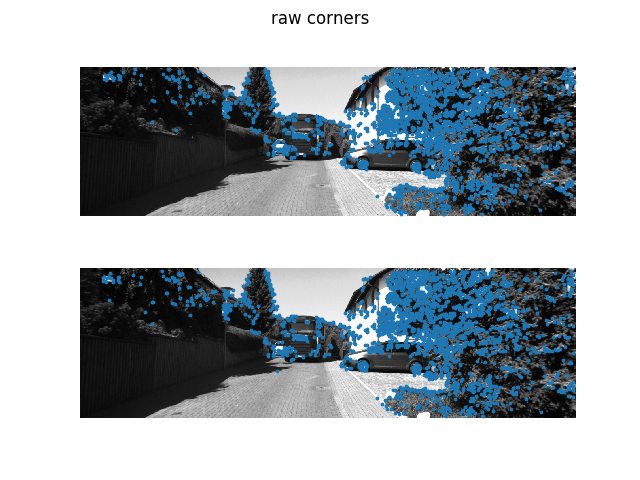
\includegraphics[width=0.9\linewidth]{10_001157_001158_raw_corners}
		\caption{Example image of the extracted corners}
		\label{fig:ex_corners}
	\end{subfigure}
	\begin{subfigure}{0.5\textwidth}
		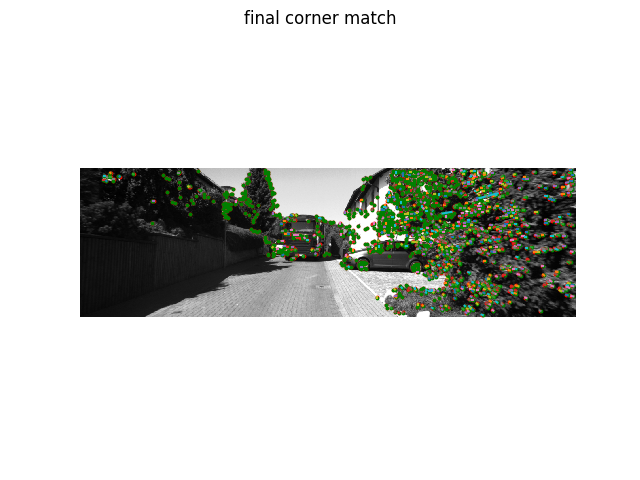
\includegraphics[width=0.9\linewidth]{10_001157_001158_final_matches}
		\caption{Example of corner matching}		
		\label{fig:ex_corner_matching}
	\end{subfigure}
	\caption{Examples of corner extraction and matching}
	\label{fig:ex_corner_and_matching}
\end{figure}

\subsection{Feature Extraction}\label{sec:features}

We bin each image into $M\times N$ grid.  For each bin in the image we
compute the histogram of corner disparities.By disparity we denote the
displacement of the corner in the image plane, e.g., if
$f_1=(x_1,y_1)$ and (the matching)
$f_2=(x_2,y_2)$ the disparity $d$ is:
\[
d = \norm{f_1-f_2} = \norm{(x_1,y_1)-(x_2,y_2)}
\]

We cross validated the different grid sizes ($N=4,5,6$ and $M=2,3,4$)
and the bin sizes $nb=100,200,300,400,500$).  Grid size of $6\times 4$
with $300$ histogram bins produced the best results (e.g. the total
feature vector length is $6*4*300=7200$).

Some statistics of the features is presented in the
Figure~\ref{fig:feature_vectors}. We expect the peaks, that correspond
to a closer image regions have a distributions shifted to the right
(i.e., larger displacements) and the peaks that correspond to a
regions farther away should be closer to zero.  This behavior can be
observed especially well for the feature vectors that correspond to
larger camera displacements (e.g. Figure~\ref{fig:1c}).

\begin{figure}[h]
	\hspace*{-4cm}
	\begin{subfigure}[b]{\linewidth}
		\centering
		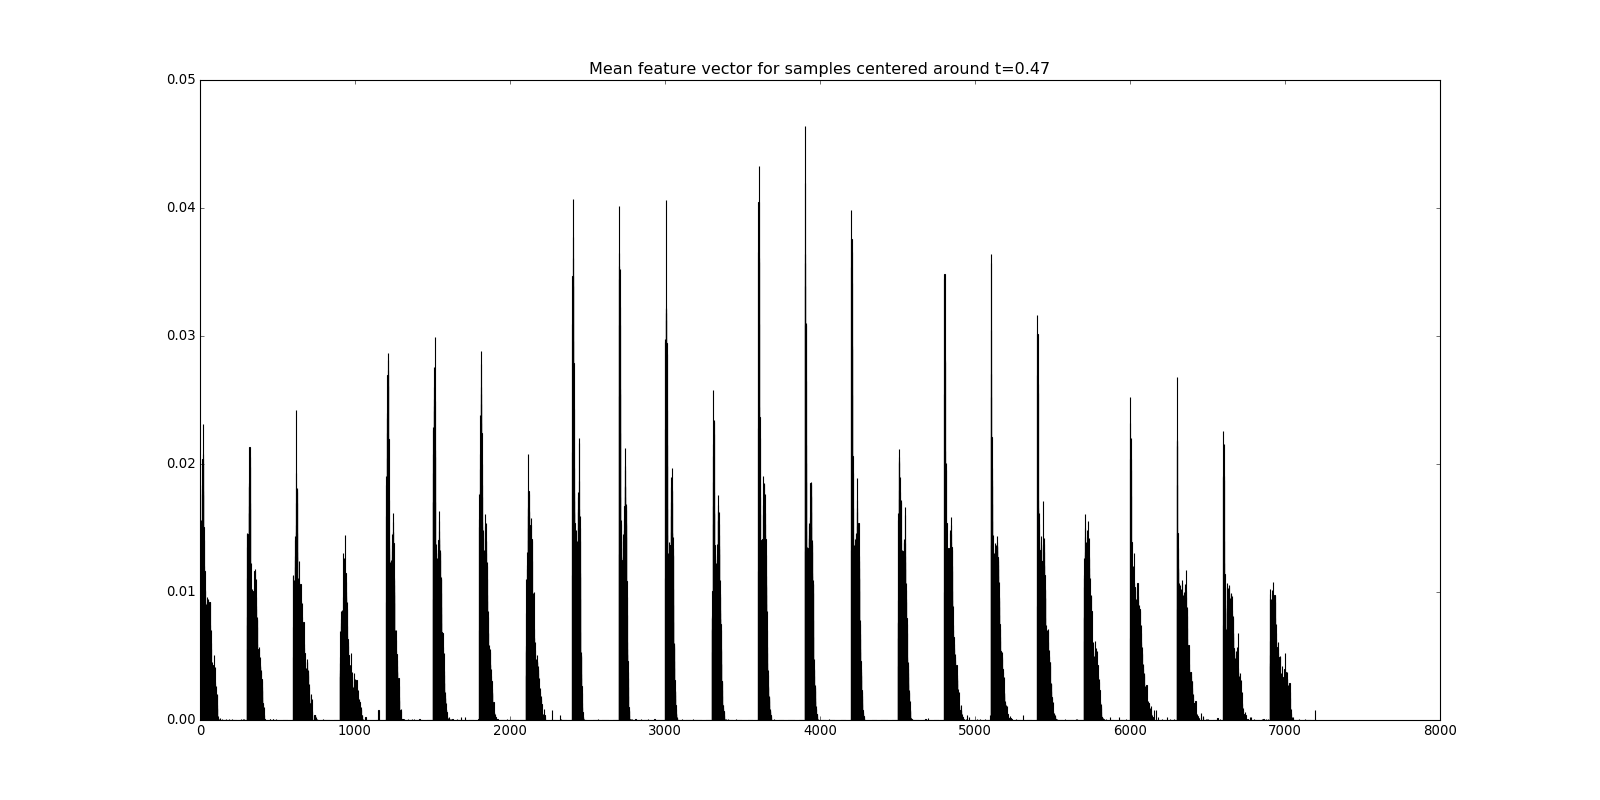
\includegraphics[width=4.0in]{00_mean_feature_vector_0_47}
		\caption{}\label{fig:1a}
	\end{subfigure}%
	\hspace*{-4cm}
	\begin{subfigure}[b]{\linewidth}
		\centering
		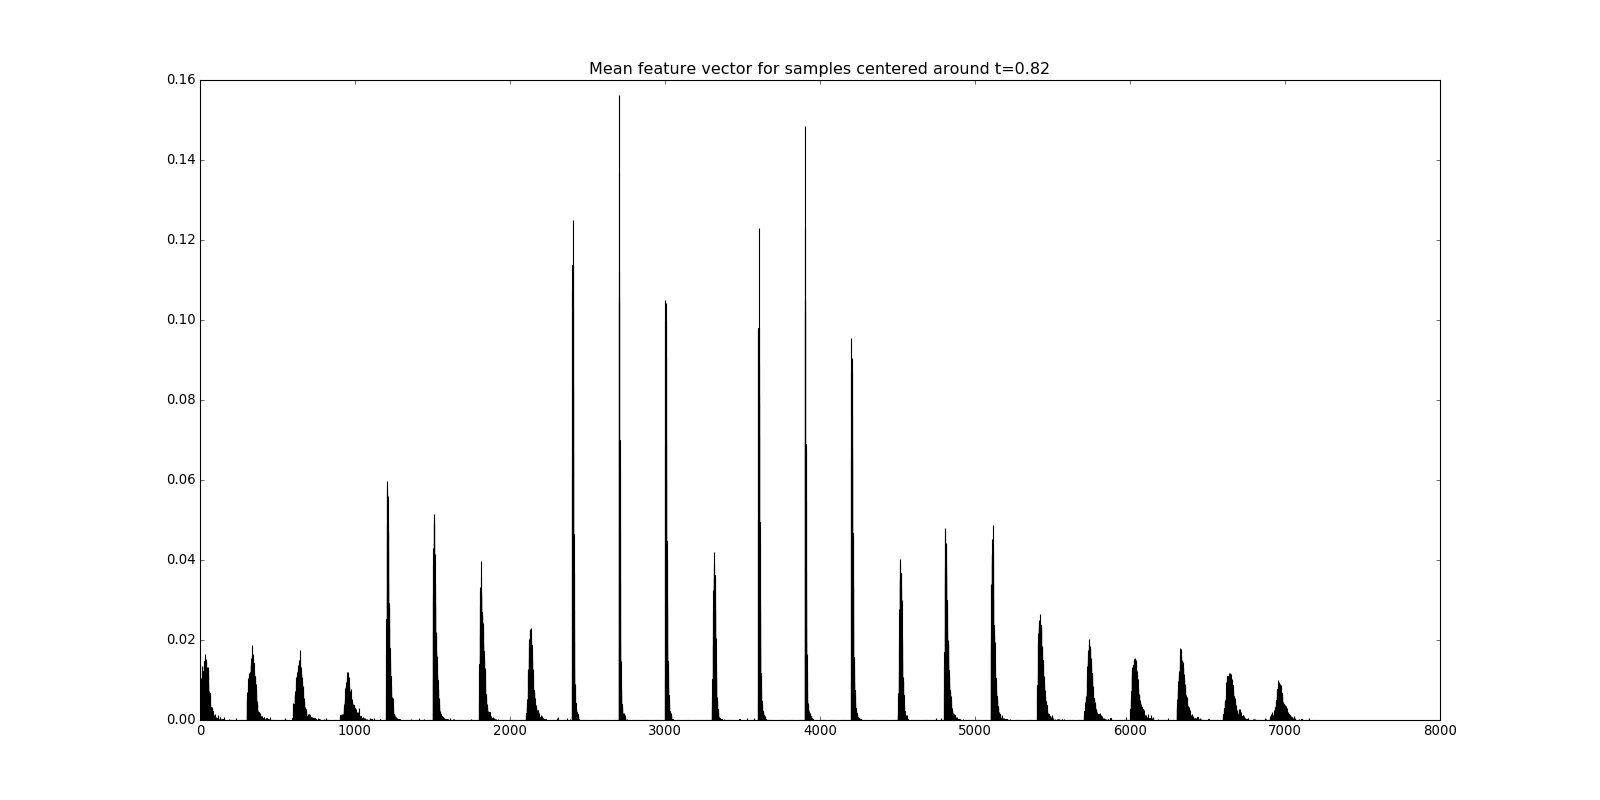
\includegraphics[width=4.0in]{00_mean_feature_vector_0_81}
		\caption{}\label{fig:1b}
	\end{subfigure}%
	\\
	\hspace*{-4cm}
	\begin{subfigure}[b]{\linewidth}
		\centering
		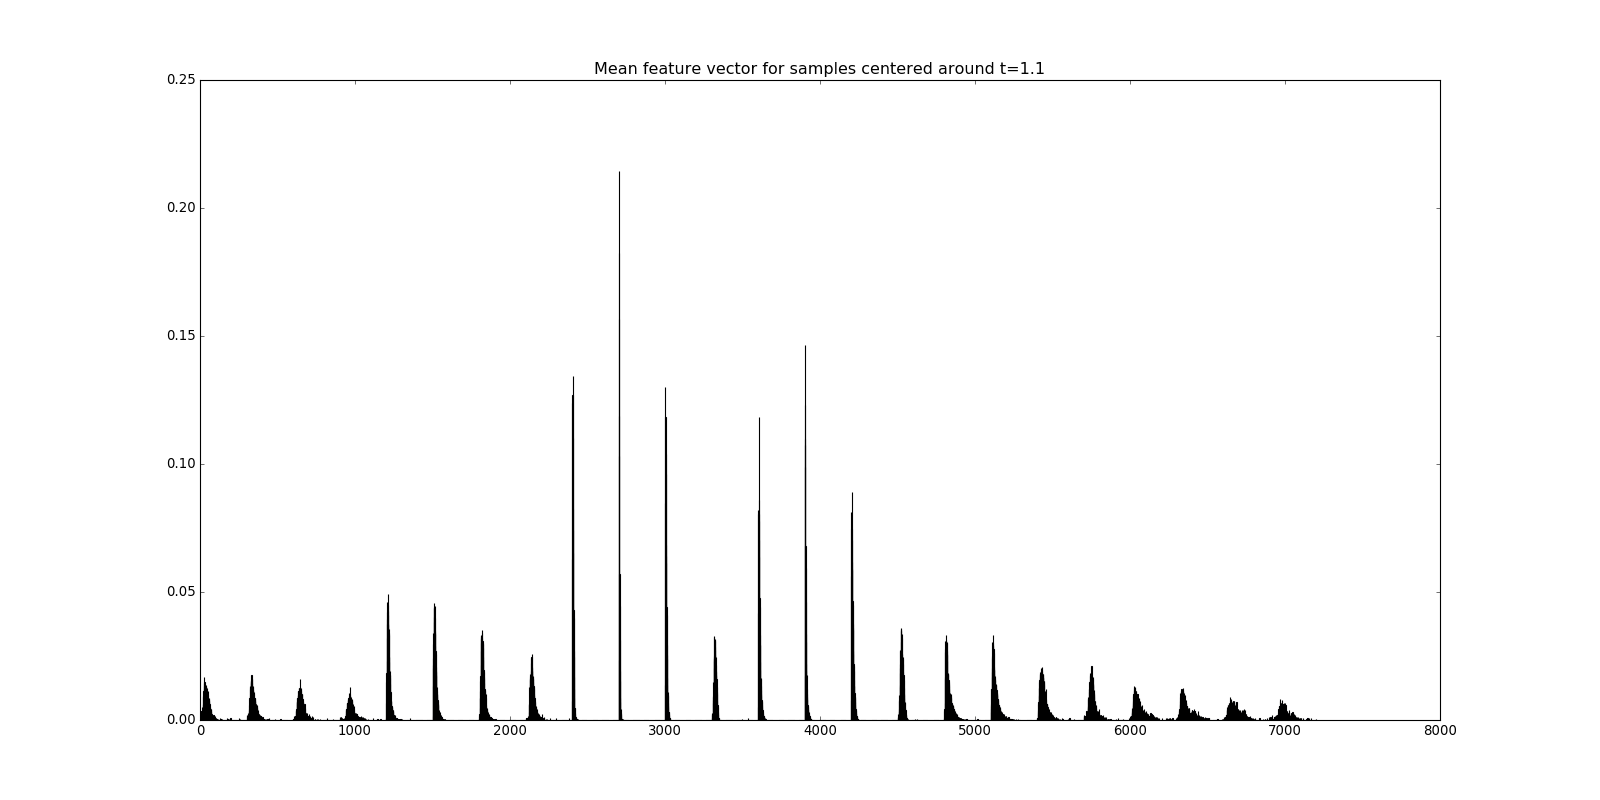
\includegraphics[width=4.0in]{00_mean_feature_vector_1_1}
		\caption{}\label{fig:1c}
	\end{subfigure}%
	\caption{Average feature vectors for samples centered around the
		specific camera translation magnitude.  Each peak corresponds to a
		grid cell (e.g. here the grid is 4 rows by 6 columns by 300 bins,
		so the feature vector is of the dimension 6*4*300=7200).  The grid
		is sampled in a column-major mode. So the first four peaks
		correspond to the leftmost column of the image grid.}
	\label{fig:feature_vectors}
\end{figure}

\section{Regression Models}

We train random forest. The implementation we use comes from the python sklearn library.  It is called extremely random tree forest.

\subsection{Results}

See Figure~\ref{fig:forest_results_images4}, ~\ref{fig:forest_results_images_no04_test}

\begin{figure}[h!]
	\begin{subfigure}{.5\textwidth}
		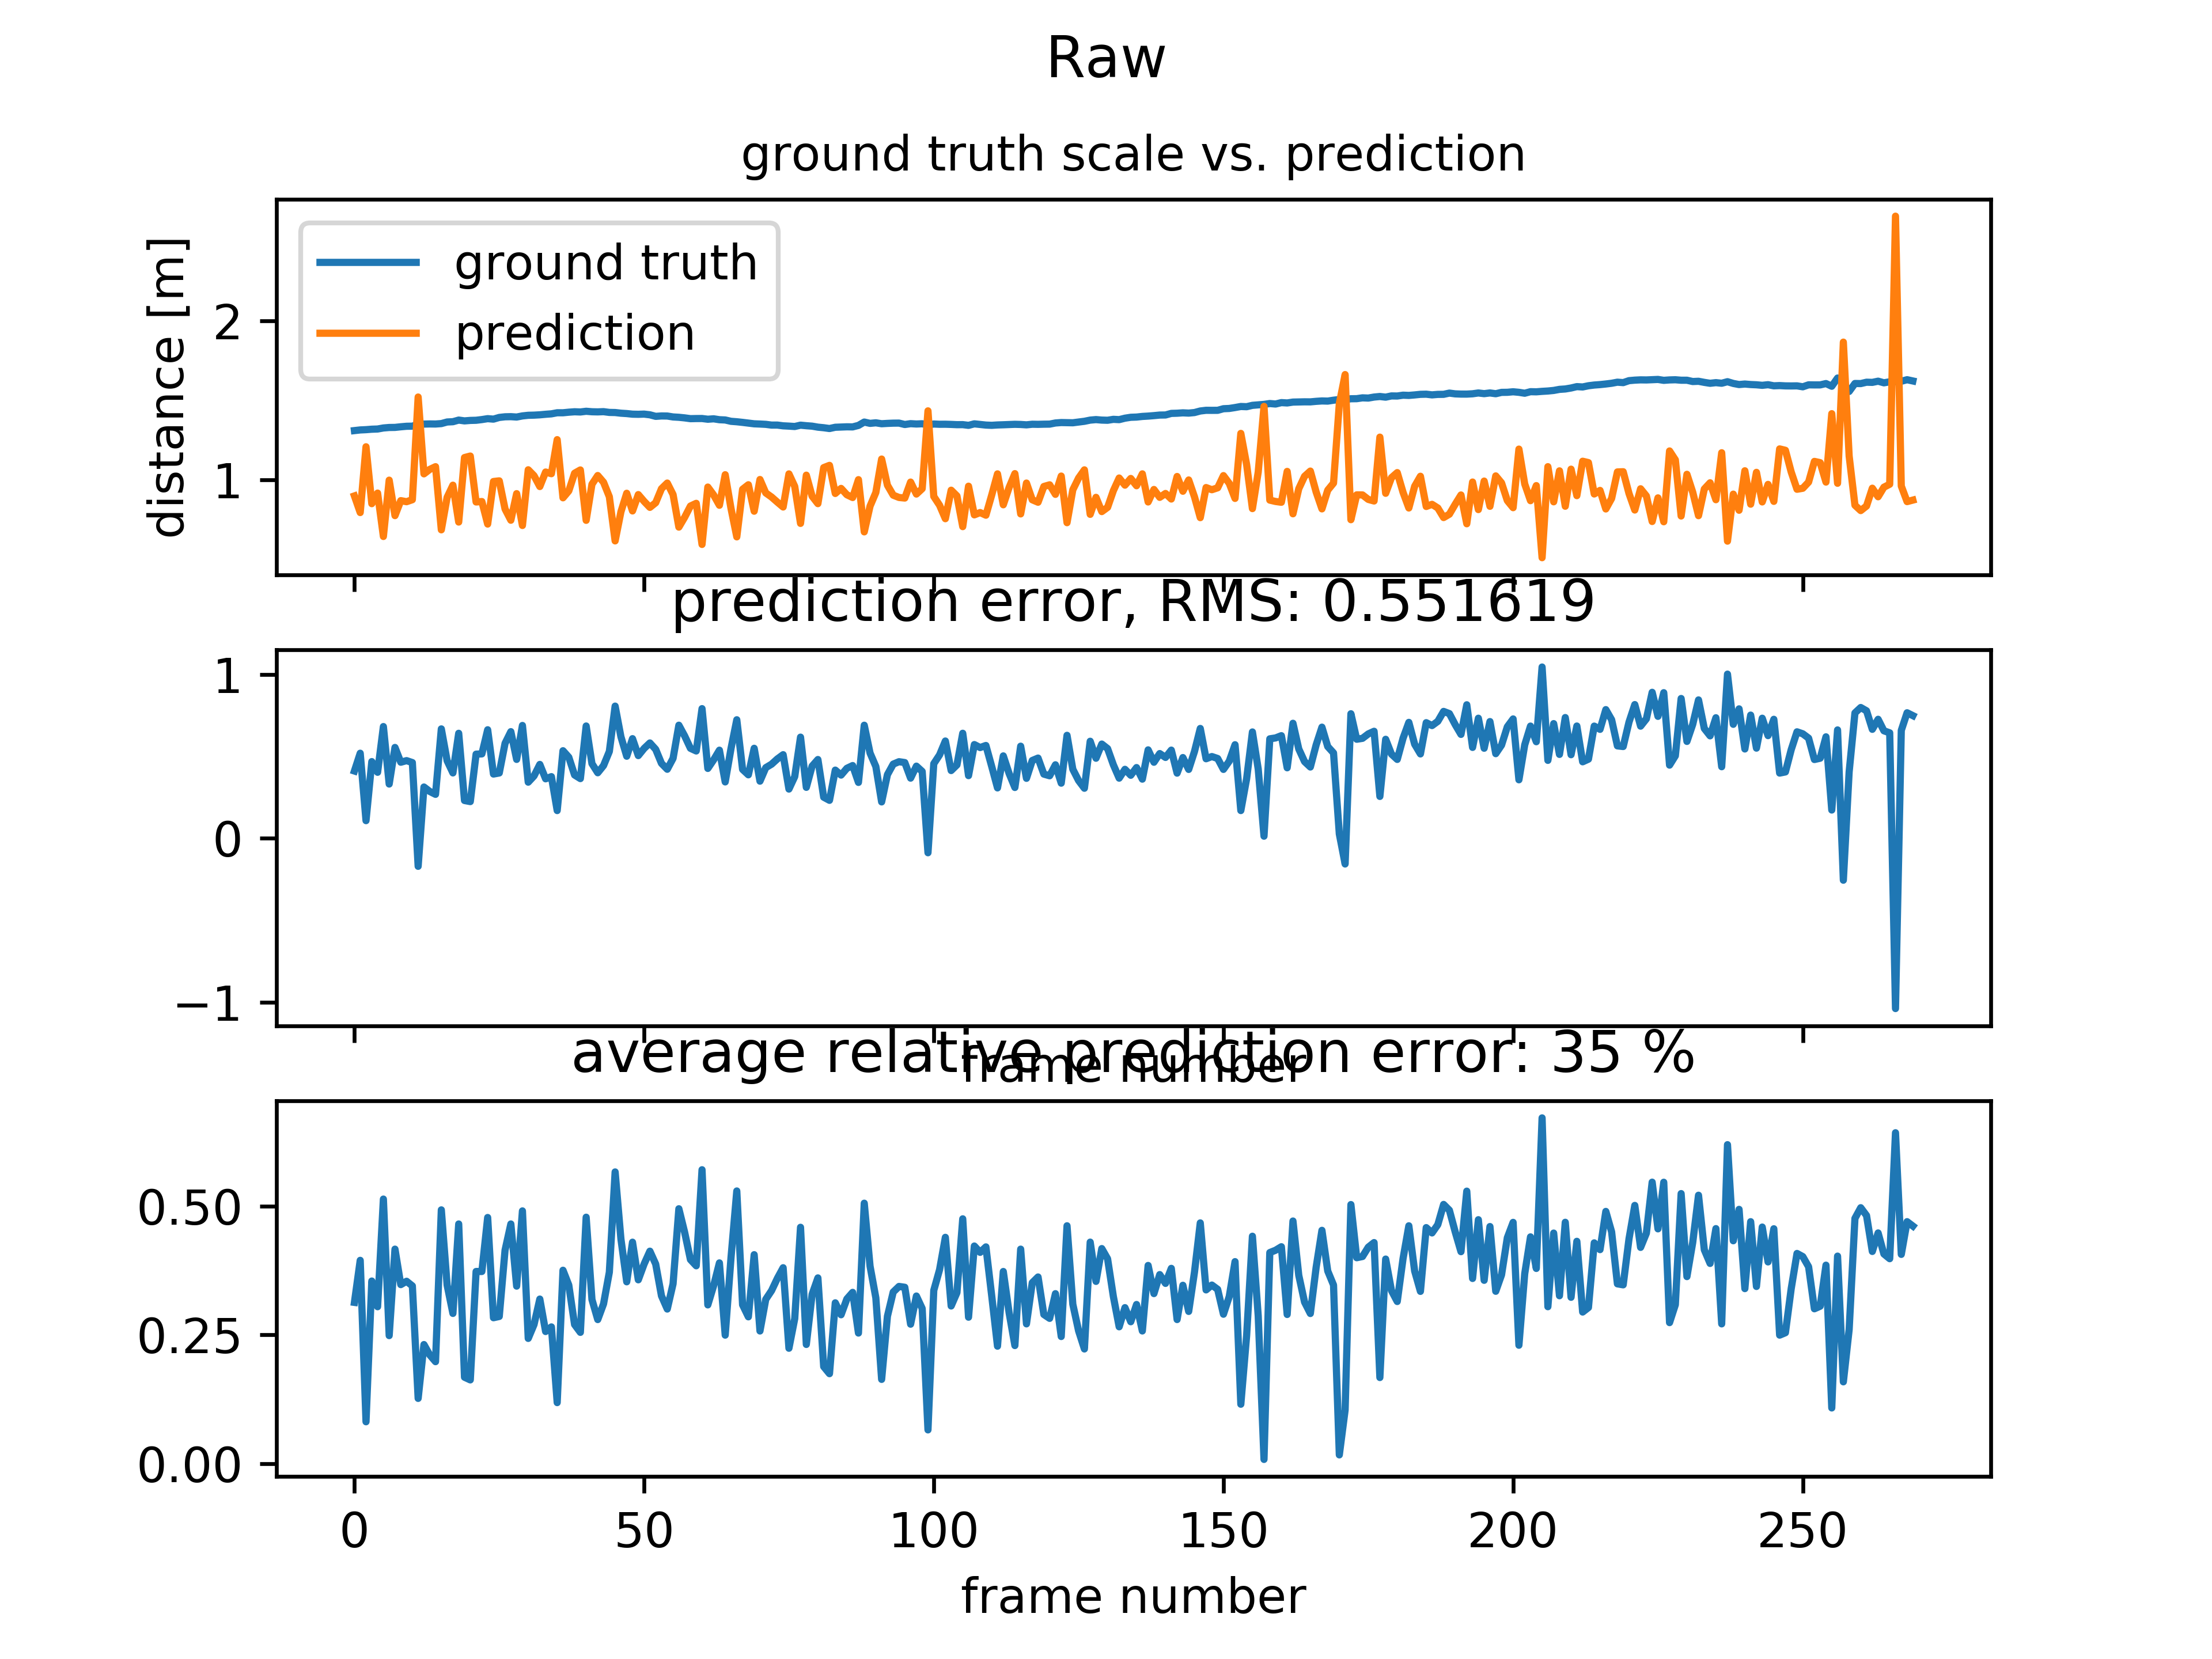
\includegraphics[width=\linewidth]{images4_test_raw}
		\caption{images04 raw}		
		\label{fig:ETR_images4_test_raw}
	\end{subfigure}
	\begin{subfigure}{.5\textwidth}
		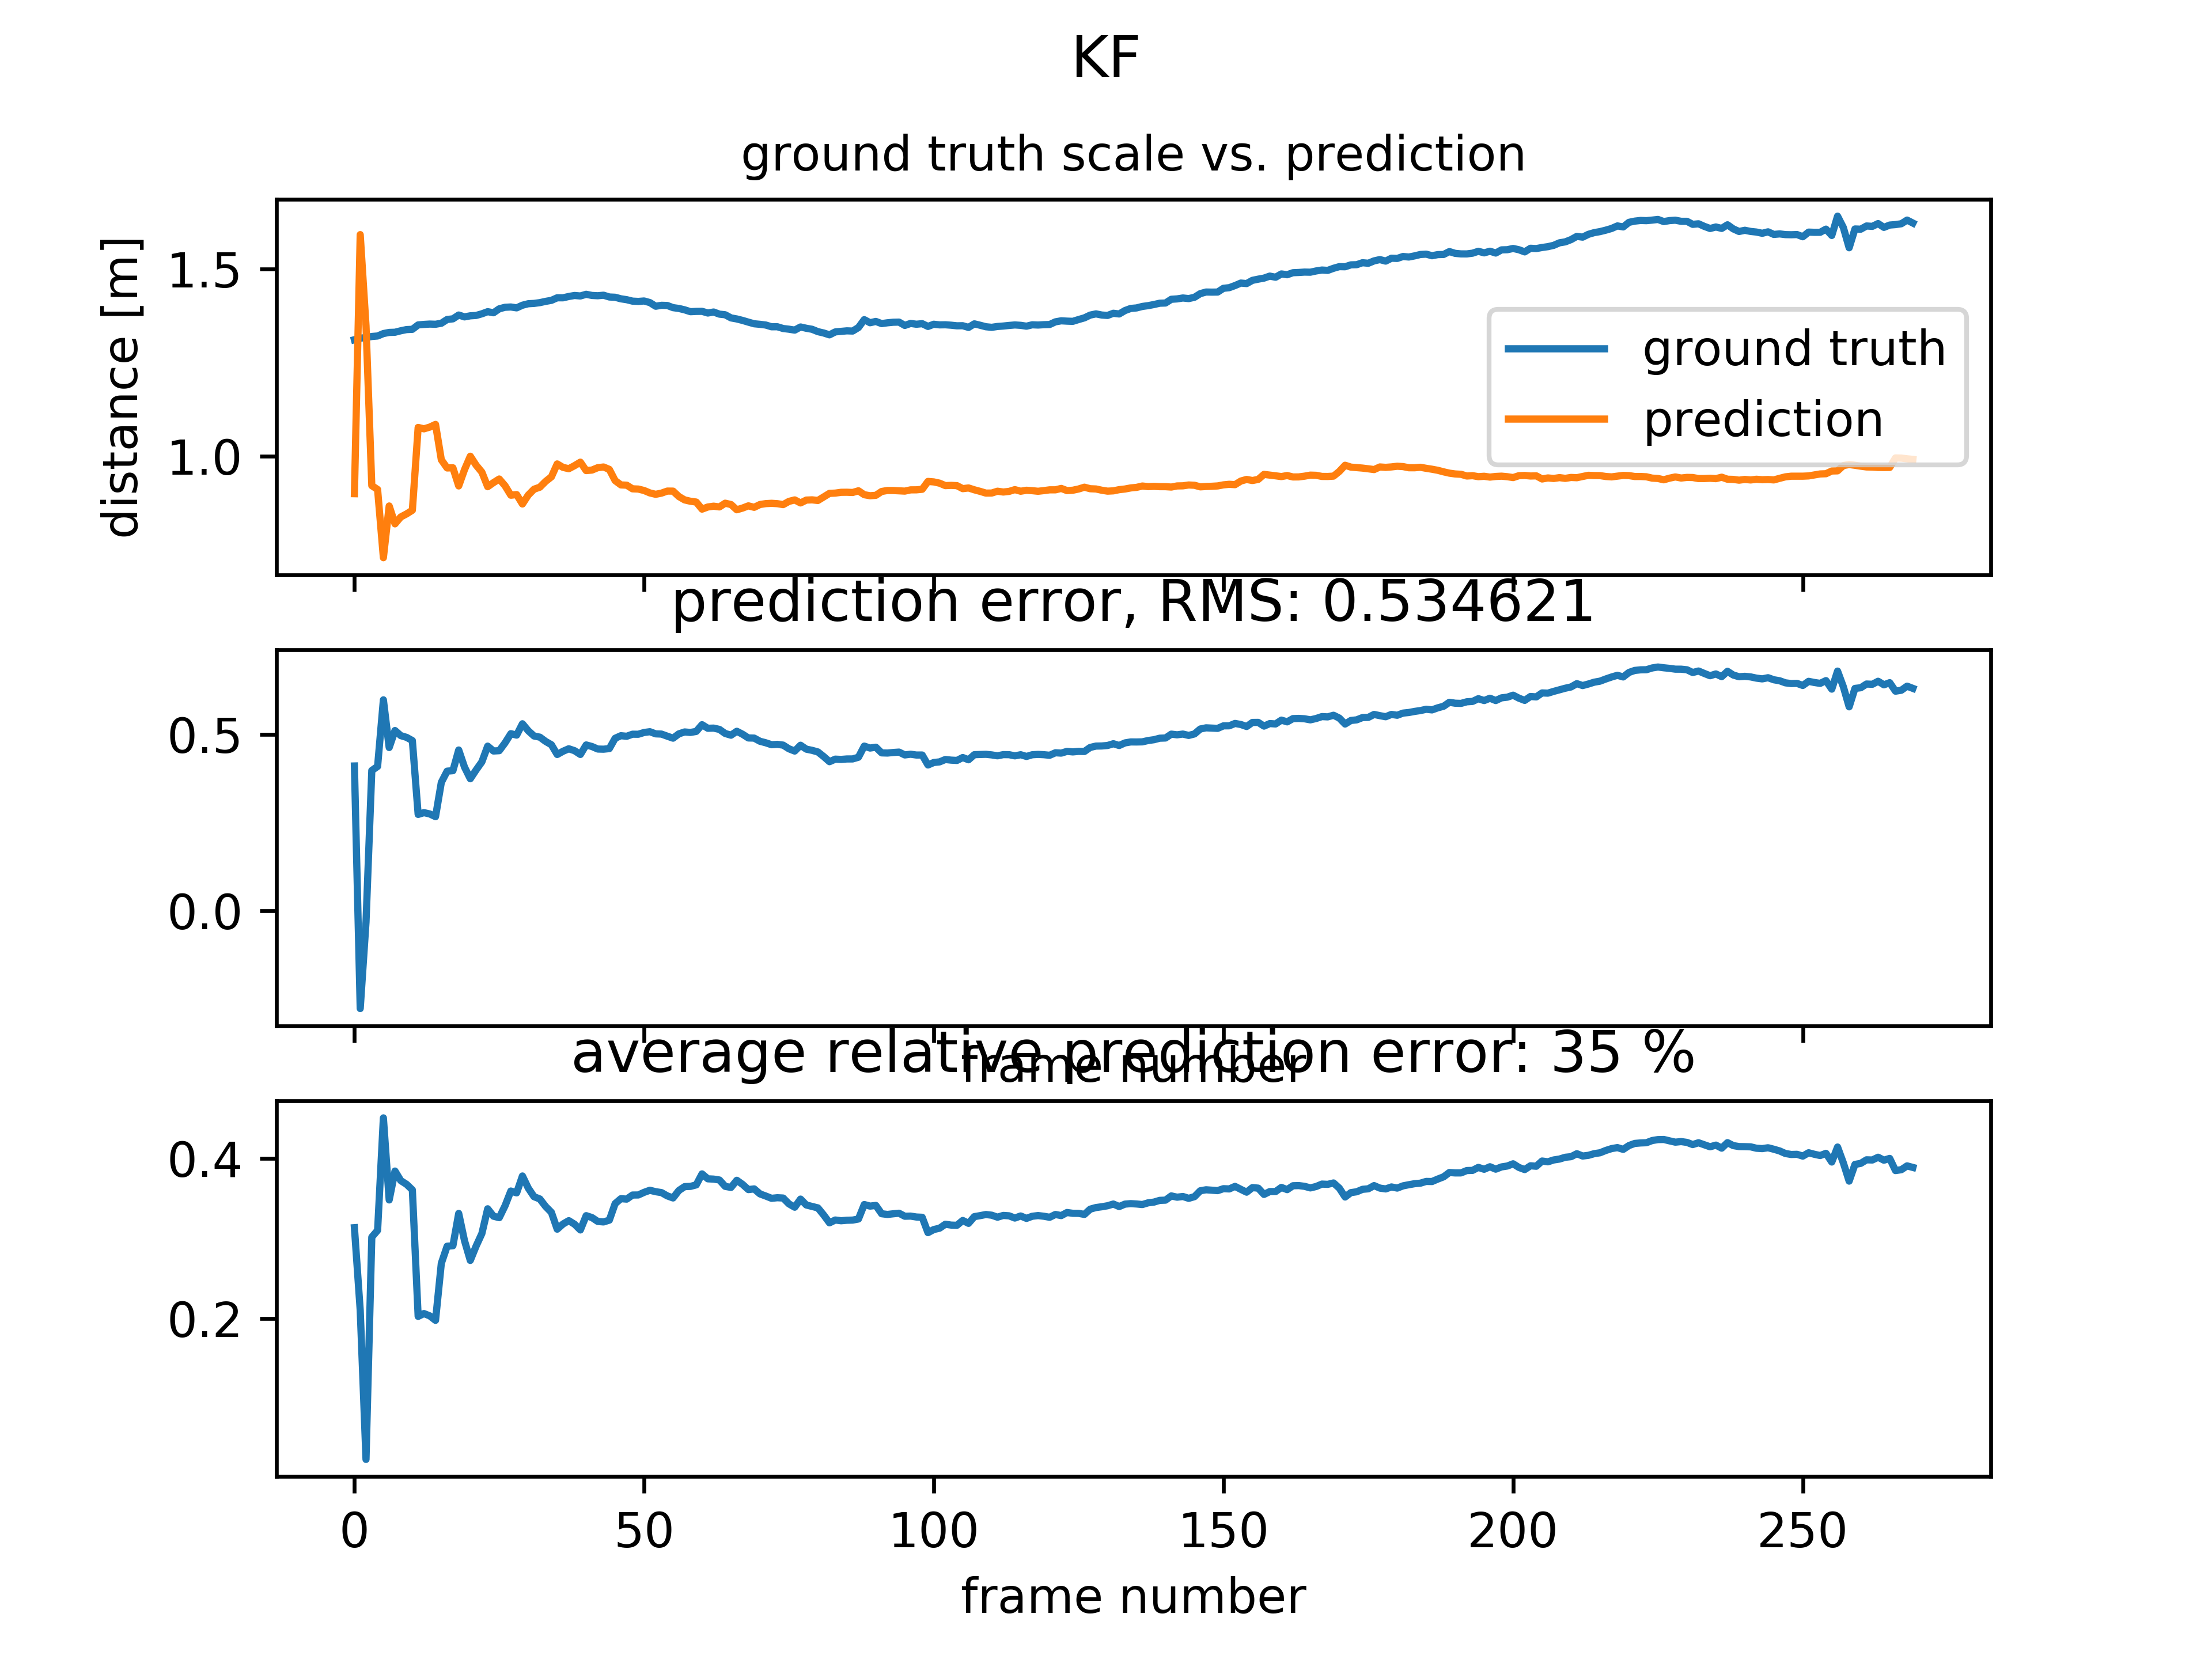
\includegraphics[width=\linewidth]{images4_test_smooth}
		\caption{images04 EKF}		
		\label{fig:images4_test_smooth}
	\end{subfigure}
	\caption{Random forest prediction evaluation for the image-set $\mathrm{images04}$}
	\label{fig:forest_results_images4}
\end{figure}

\begin{figure}[h!]
	\begin{subfigure}{.5\textwidth}
		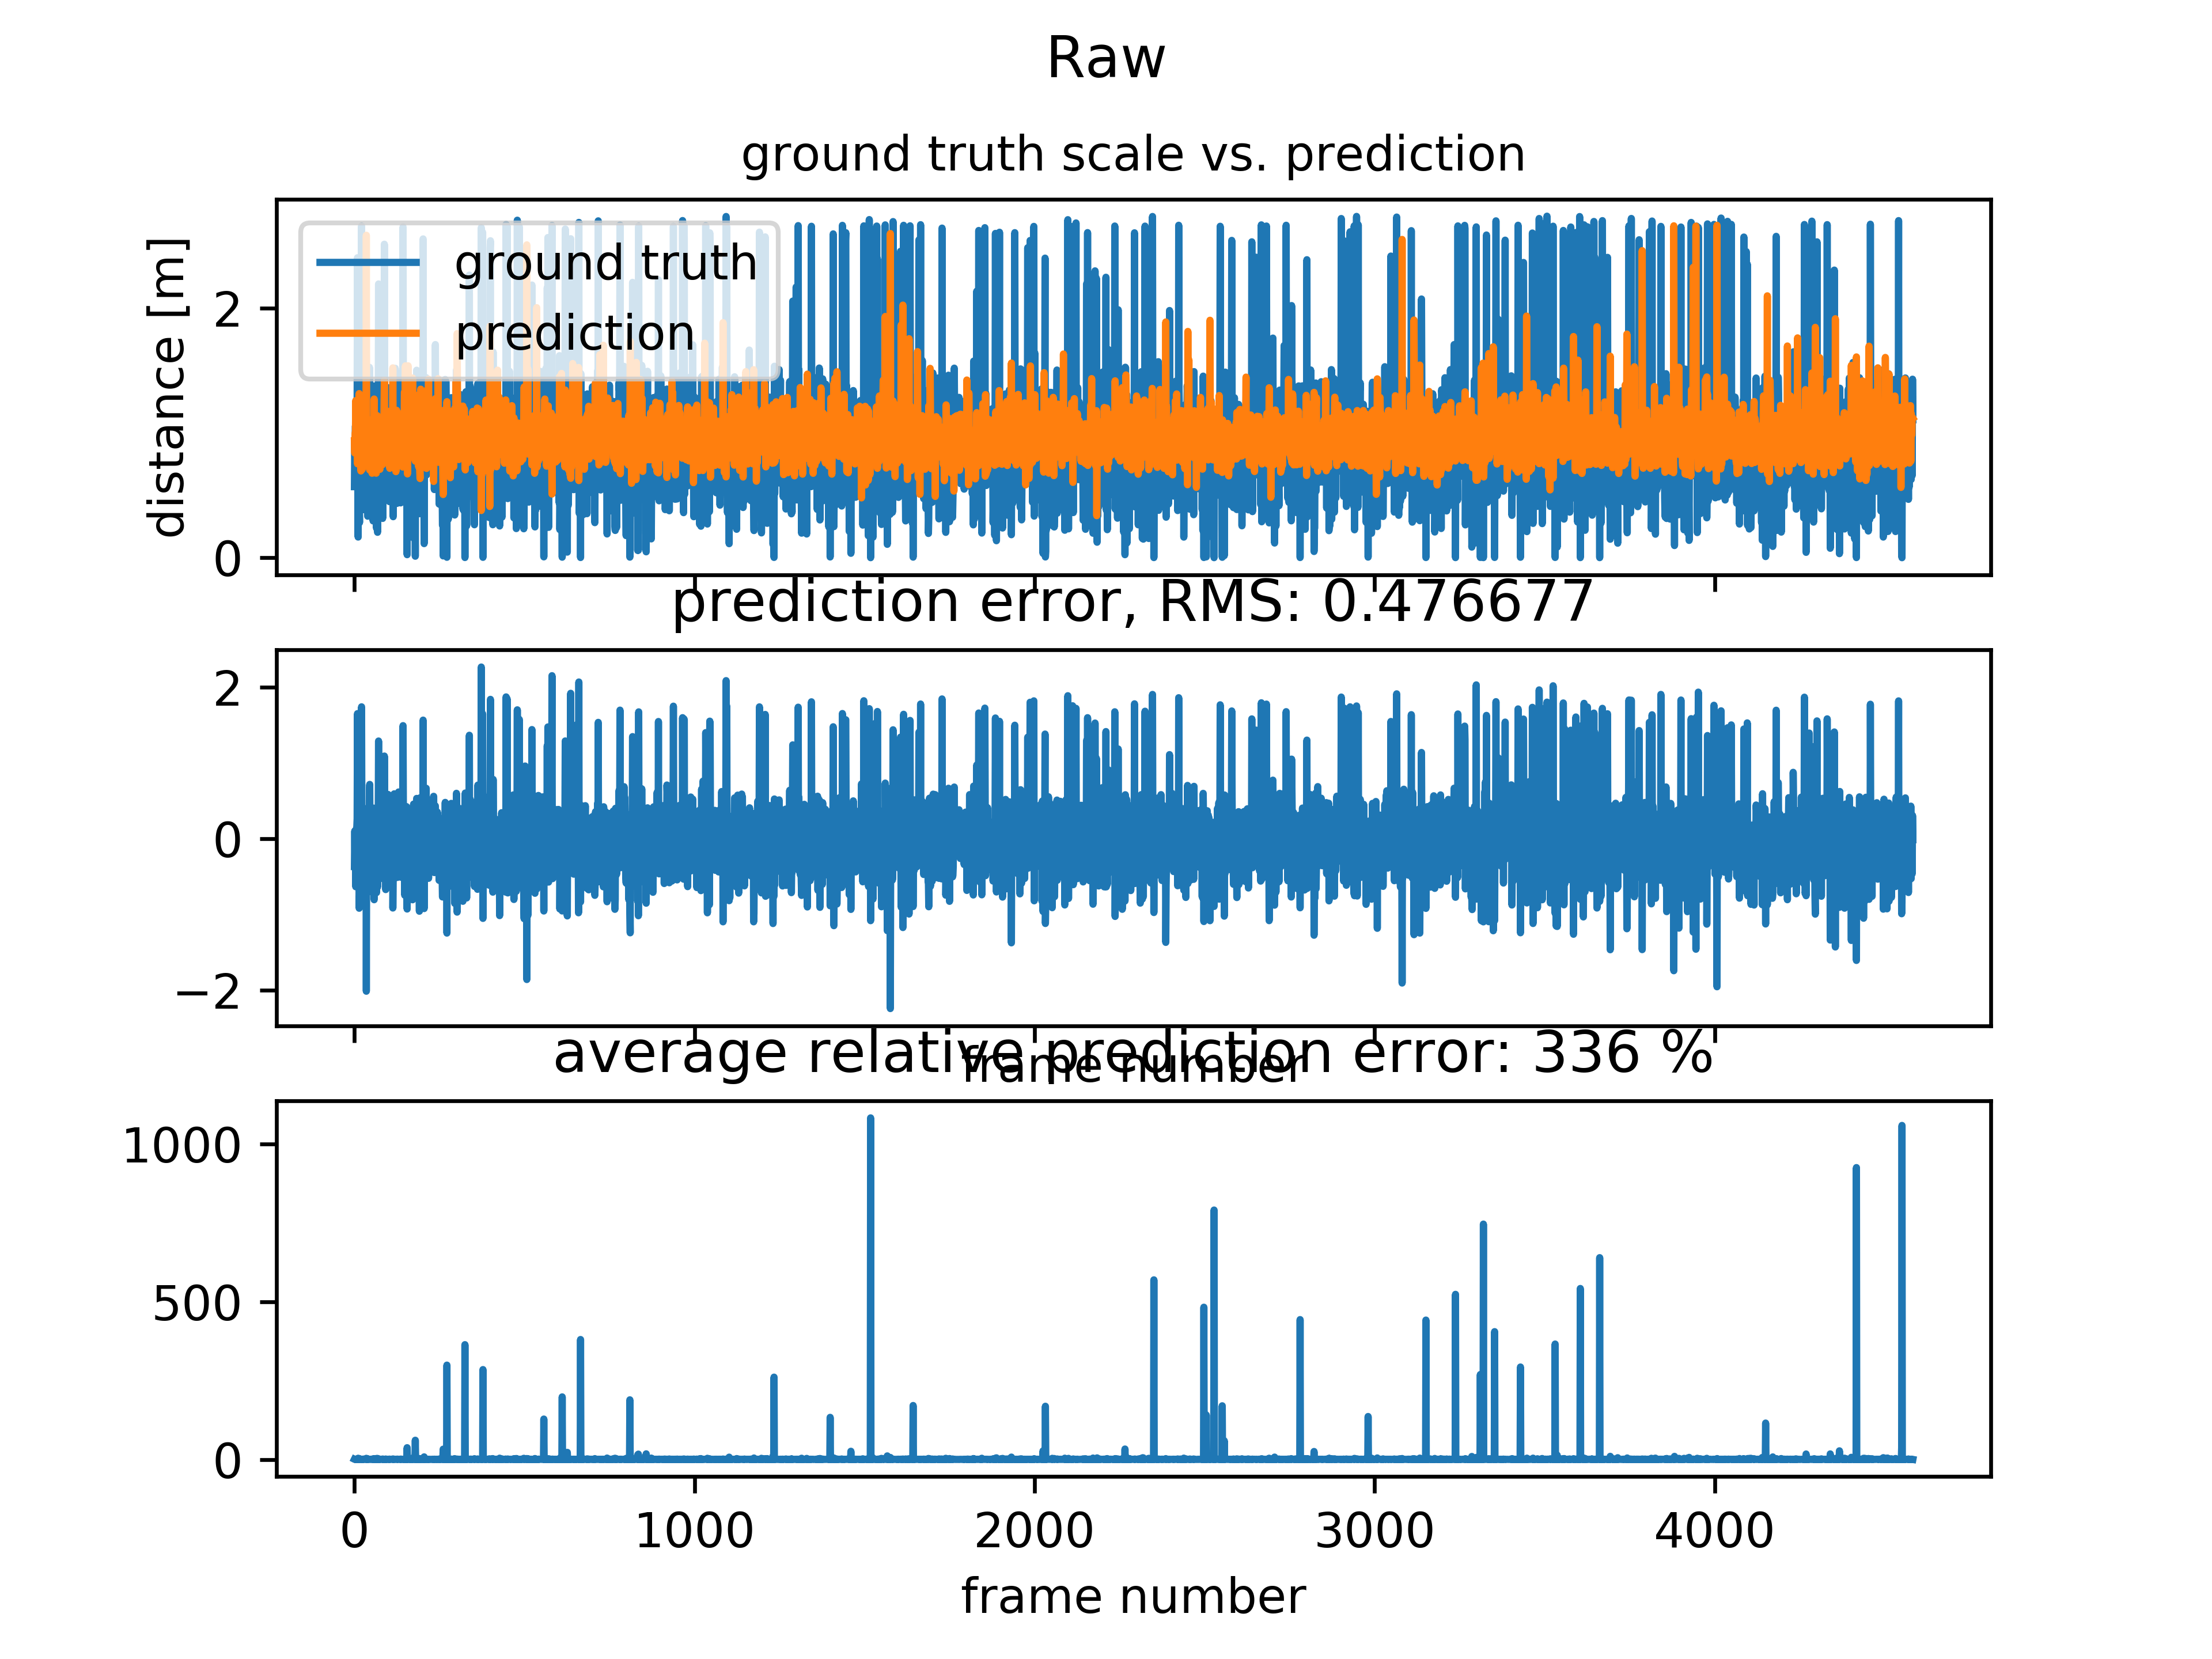
\includegraphics[width=\linewidth]{images_no04_test_raw}
		\caption{images\_no04\_test}
		\label{fig:ETR_images_no04_test}
	\end{subfigure}
	\caption{Random forest prediction evaluation for the image-set $\mathrm{images\_no04\_test}$}
	\label{fig:forest_results_images_no04_test}
\end{figure}

\section{Convolutional neural networks}

We also explore convolutional neural networks as a regressor for our
task.  The choice of the architecture is influenced
by~\cite{fischer2015flownet}.

\subsection{Architecture choice}
TBD

\subsection{Results}
See Figures~\ref{fig:ZF_results_images4},~\ref{fig:ZF_results_images_no04_test}

\begin{figure}[h!]
	\begin{subfigure}{.5\textwidth}
		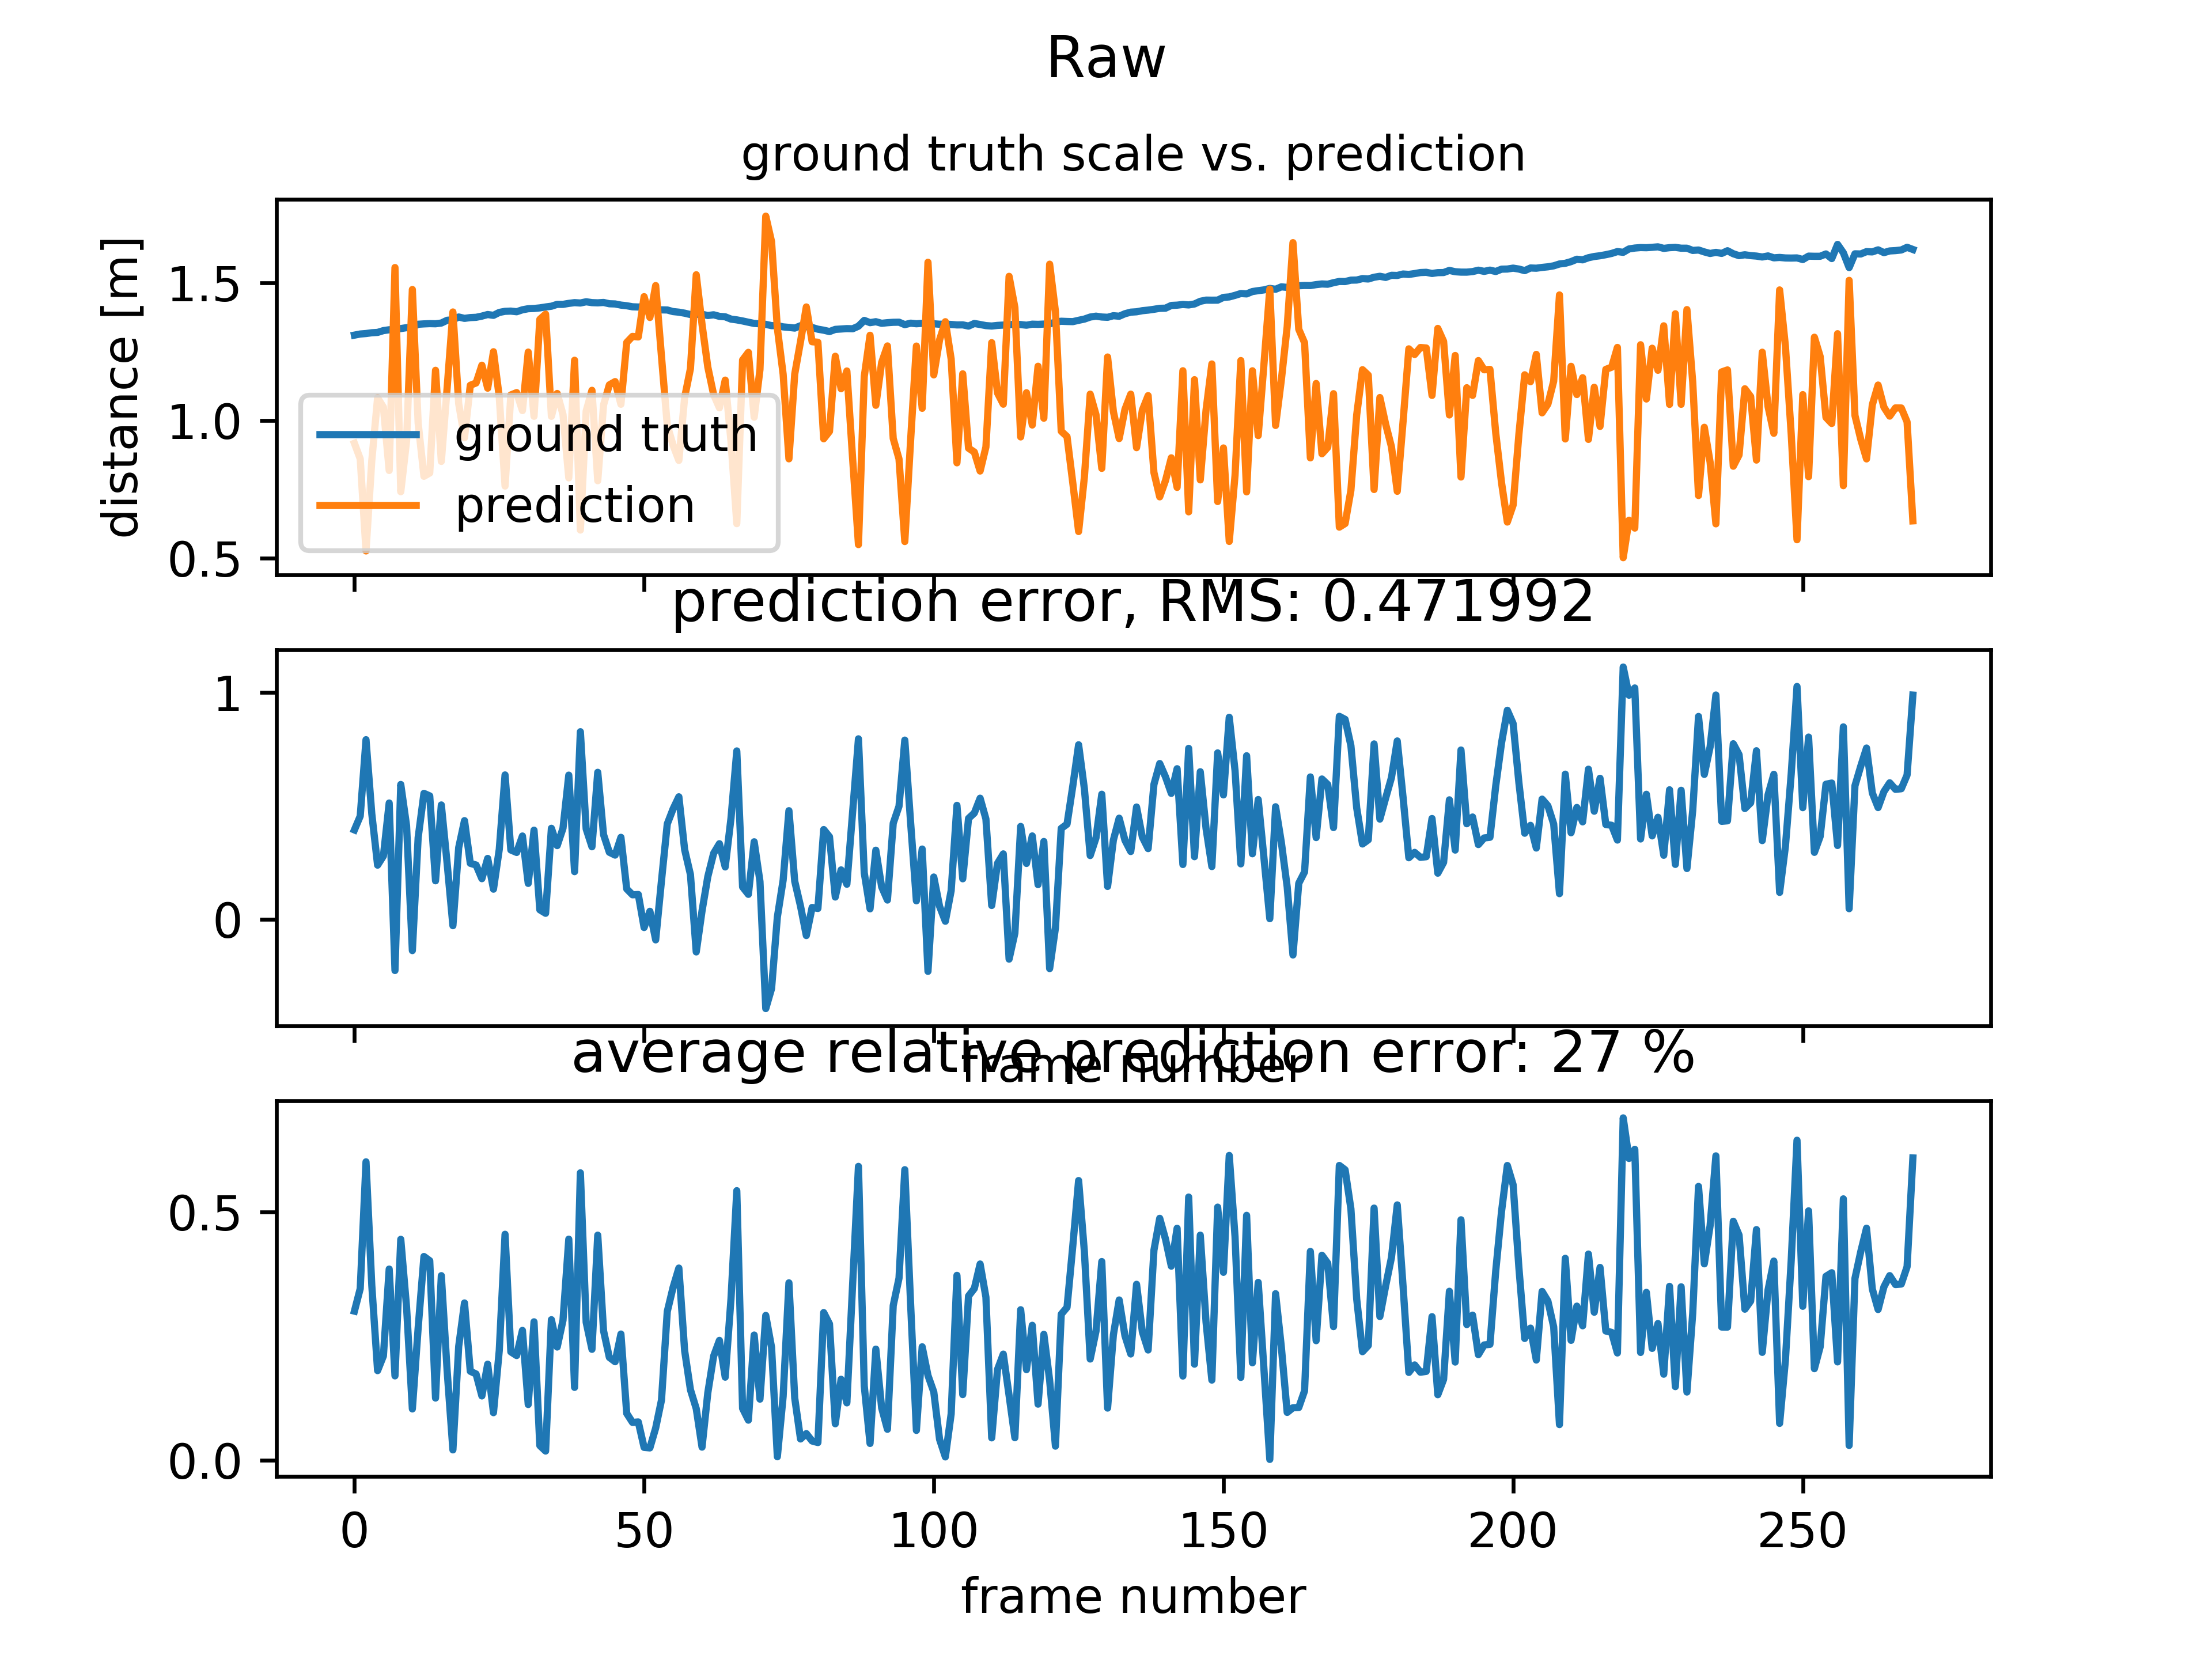
\includegraphics[width=\linewidth]{images4_test_ZF_raw}
		\caption{images04 raw}		
		\label{fig:ZF_images4_test_raw}
	\end{subfigure}
	\begin{subfigure}{.5\textwidth}
		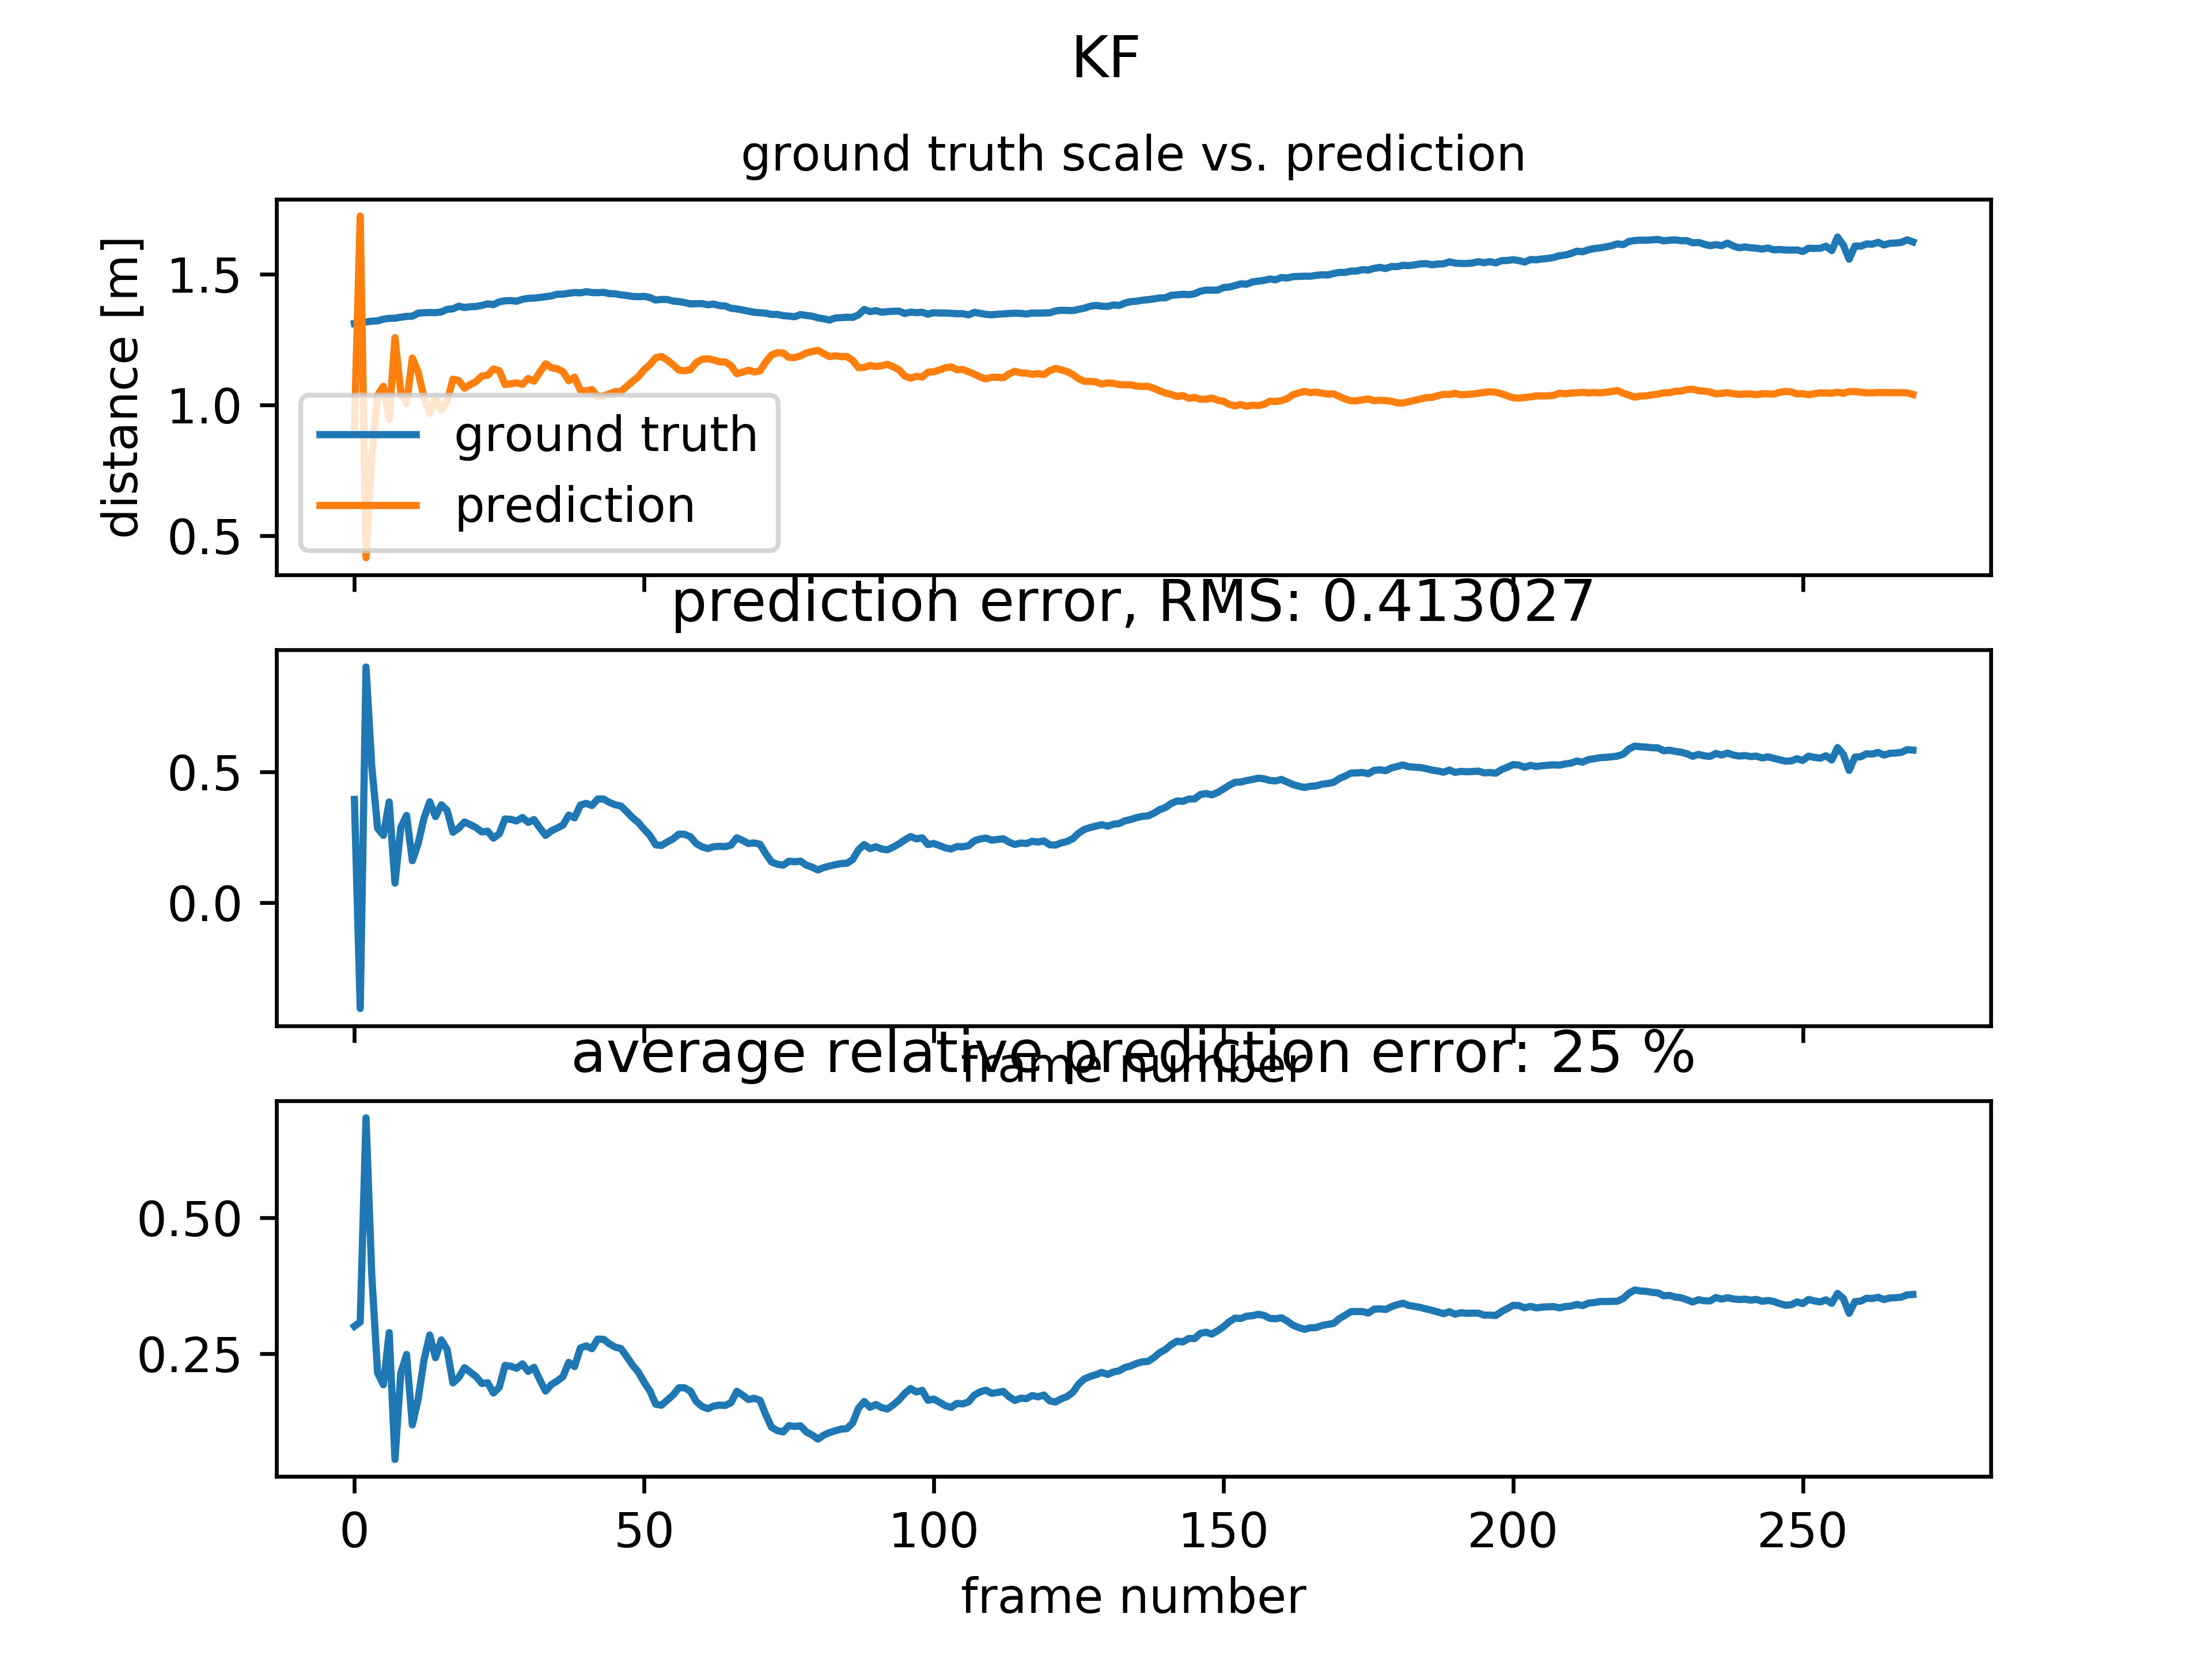
\includegraphics[width=\linewidth]{images4_test_ZF_smooth}
		\caption{images04 EKF}		
		\label{fig:ZF_images4_test_smooth}
	\end{subfigure}
	\caption{ZF prediction evaluation for the image-set $\mathrm{images04}$}
	\label{fig:ZF_results_images4}
\end{figure}

\begin{figure}[h!]
	\begin{subfigure}{.5\textwidth}
		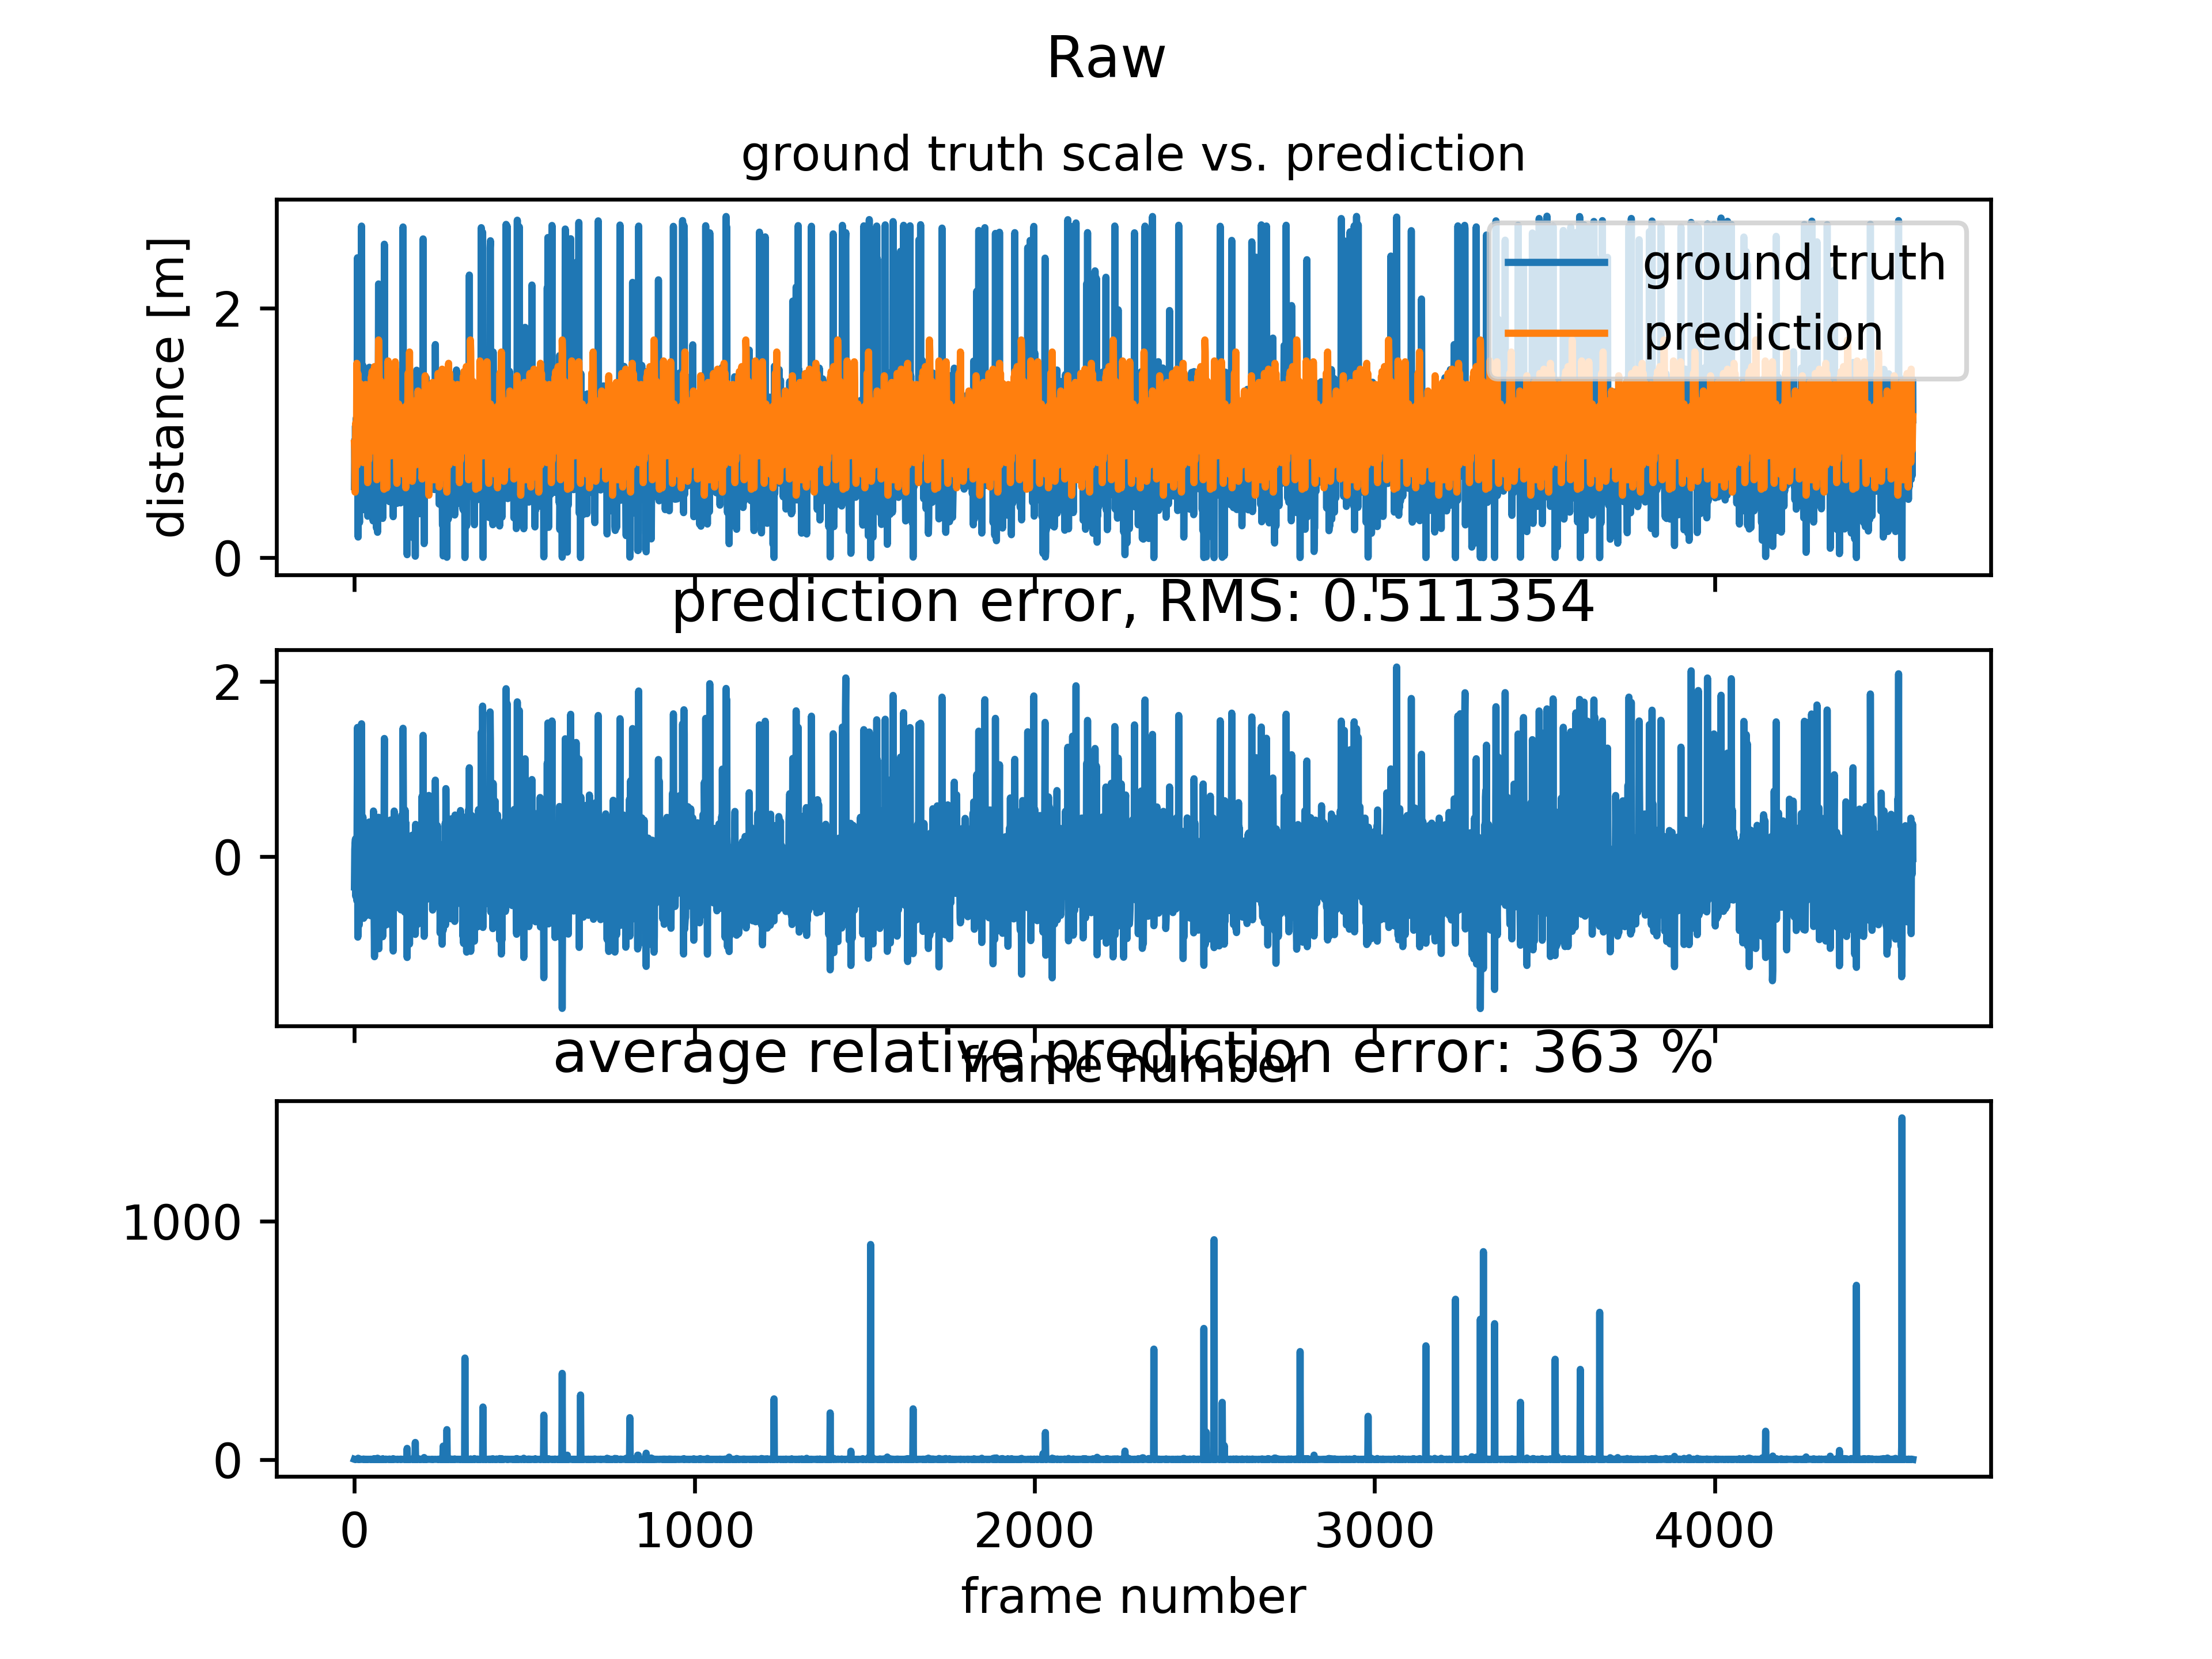
\includegraphics[width=\linewidth]{images_no04_test_ZF_raw}
		\caption{images\_no04\_test}
		\label{fig:ZF_images_no04_test_raw}
	\end{subfigure}
	\caption{ZF prediction evaluation for the image-set $\mathrm{images\_no04\_test}$}
	\label{fig:ZF_results_images_no04_test}
\end{figure}

\subsection{Experiments}
\subsection{The dataset}

We train and test on the KITTI dataset. There are 11 sequences with
the vehicle motion ground truth (DGPS).  We organize our data like follows:

\begin{itemize}
	\item Arbitrarily choose sequence 04 for testing (image-set $\mathrm{images04}$).  This image-set contains subsequent camera frames (e.g. the subsequent images are highly correlated)
	\item Split the remaining data into the train set (image-set $\mathrm{images\_no04}$) and the test set (image-set $\mathrm{images\_no04\_test}$).  These train/test sets are created after randomly shuffling the data.
\end{itemize}

The statistics of the scales for the above image-sets are in Figure~\ref{fig:scale_stats} (most of the mass is around 1.0 meter, which makes it about 36 km/h, since the sequences are captured at 10 fps).

\begin{figure}[h!]
	\begin{subfigure}{0.5\textwidth}
		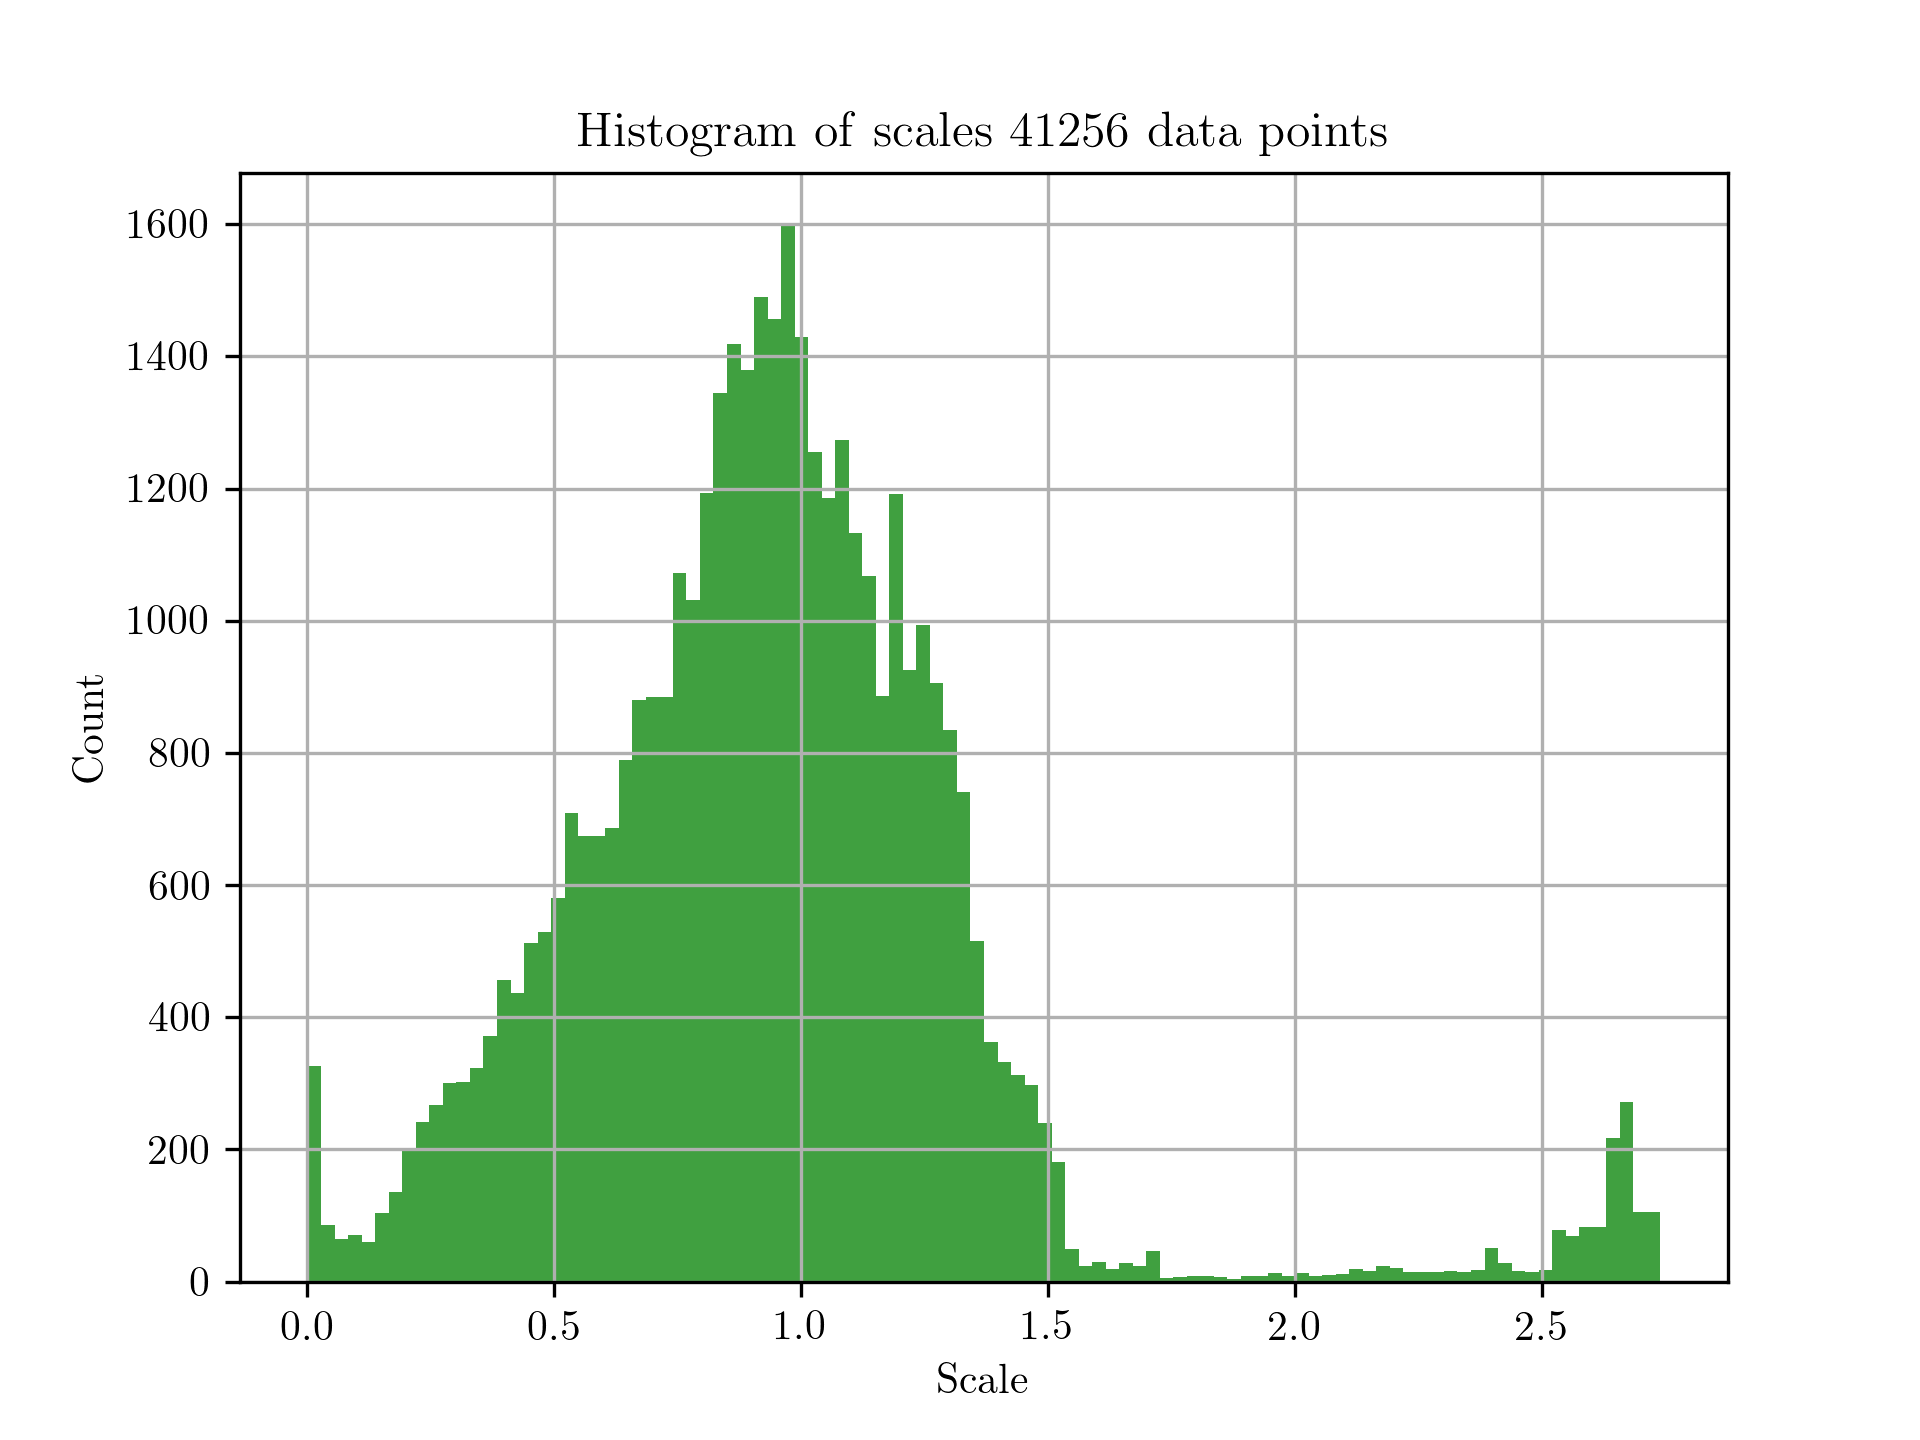
\includegraphics[width=0.9\linewidth]{stats_images_no04_rgb_shuf}
		\caption{images\_no04}		
		\label{fig:stats_images_no04_rgb_shuf}
	\end{subfigure}
	\begin{subfigure}{0.5\textwidth}
		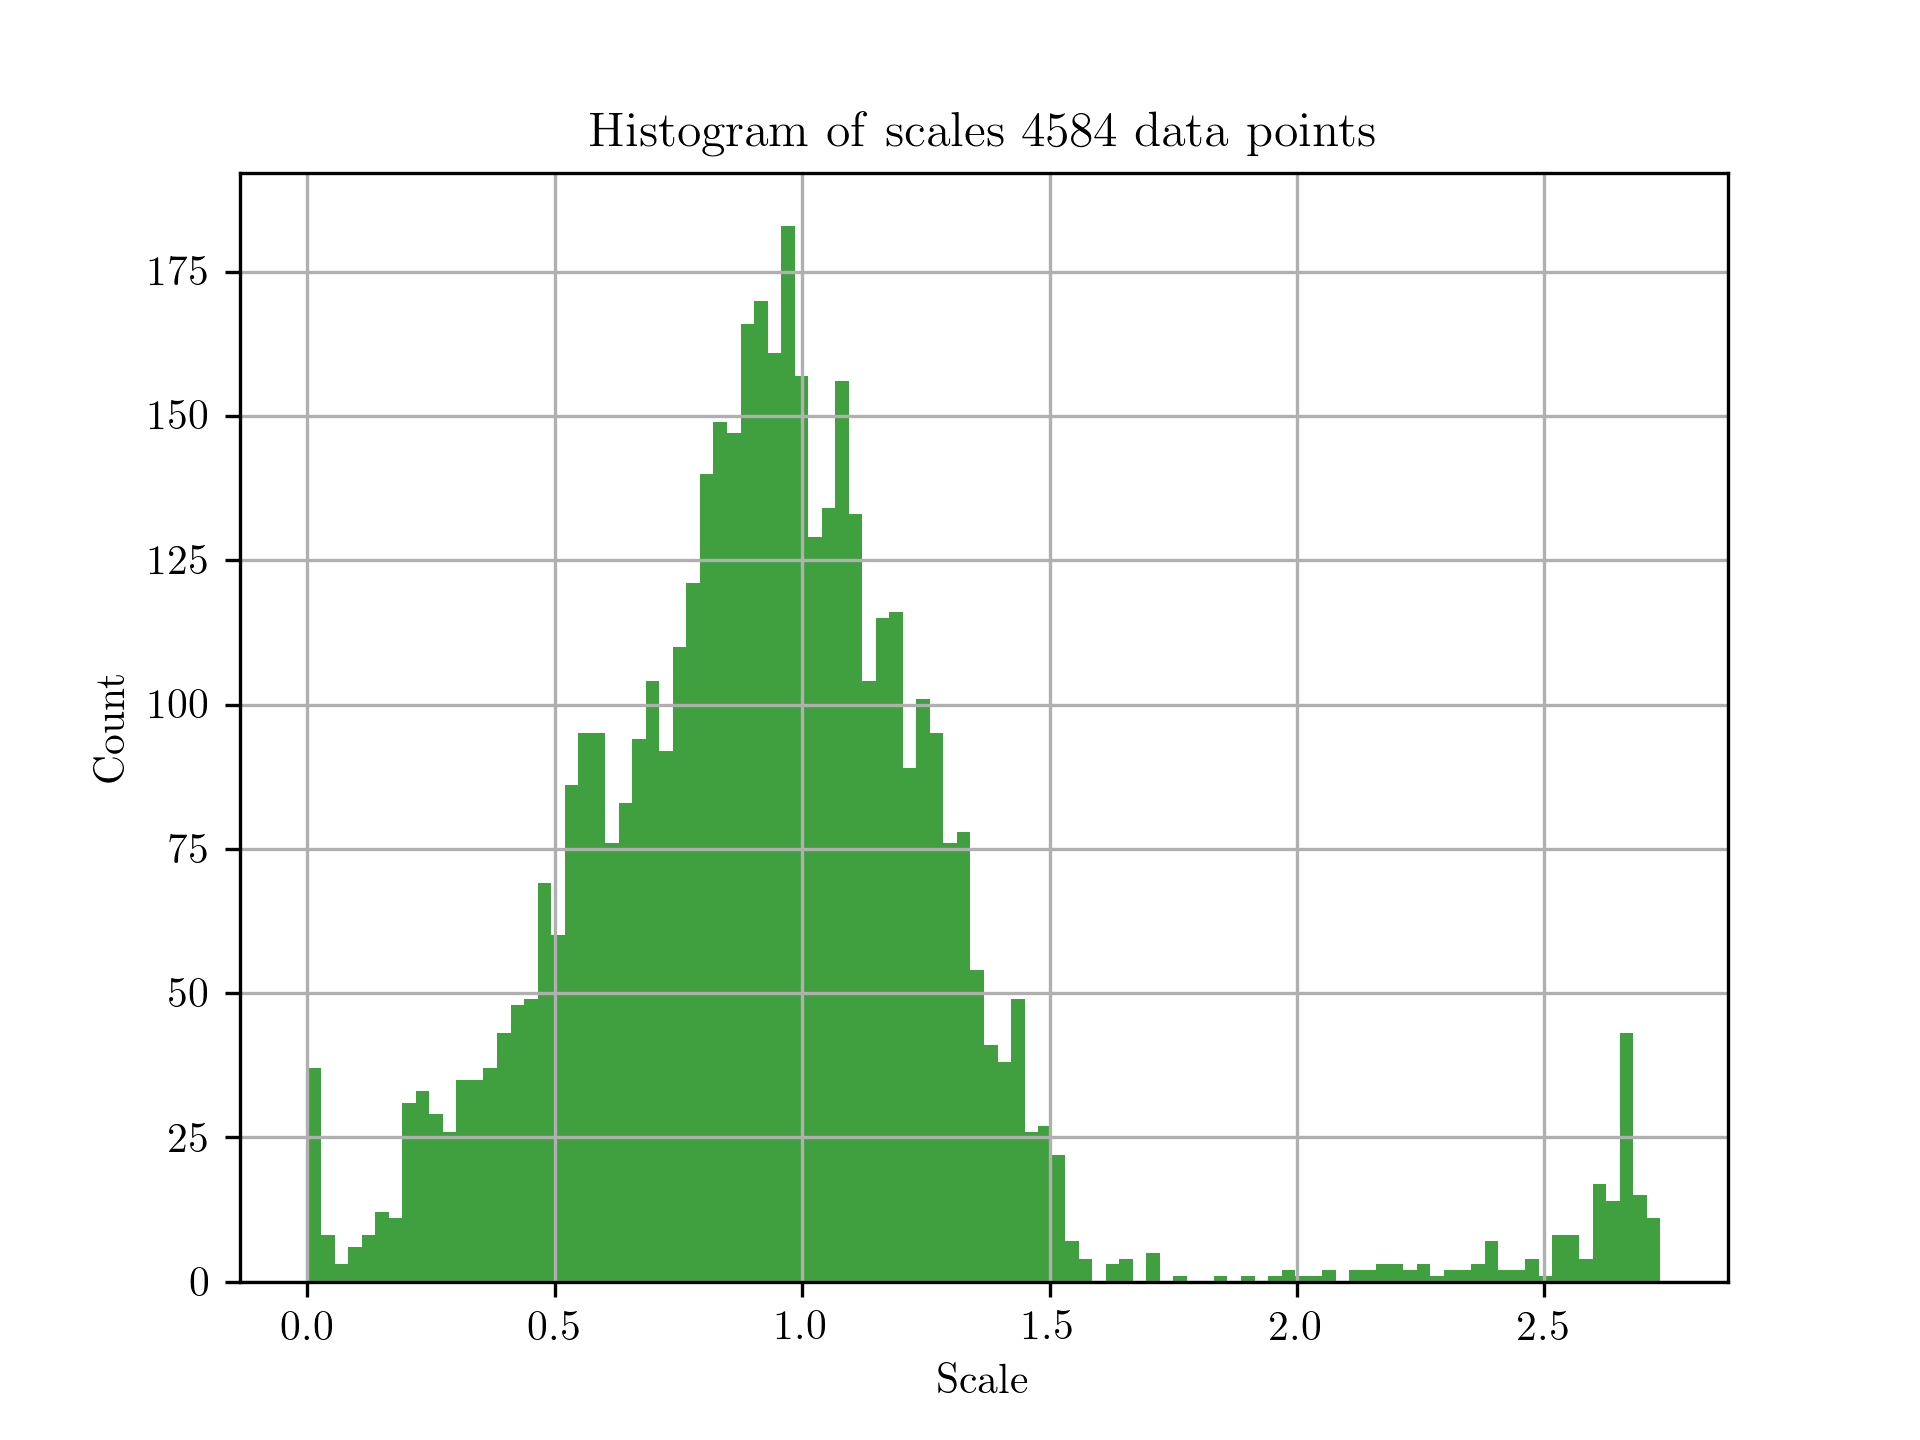
\includegraphics[width=0.9\linewidth]{stats_images_no04_rgb_test_shuf}
		\caption{images\_no04\_test}		
		\label{fig:stats_images_no04_rgb_test_shuf}
	\end{subfigure}
	\begin{subfigure}{0.5\textwidth}
		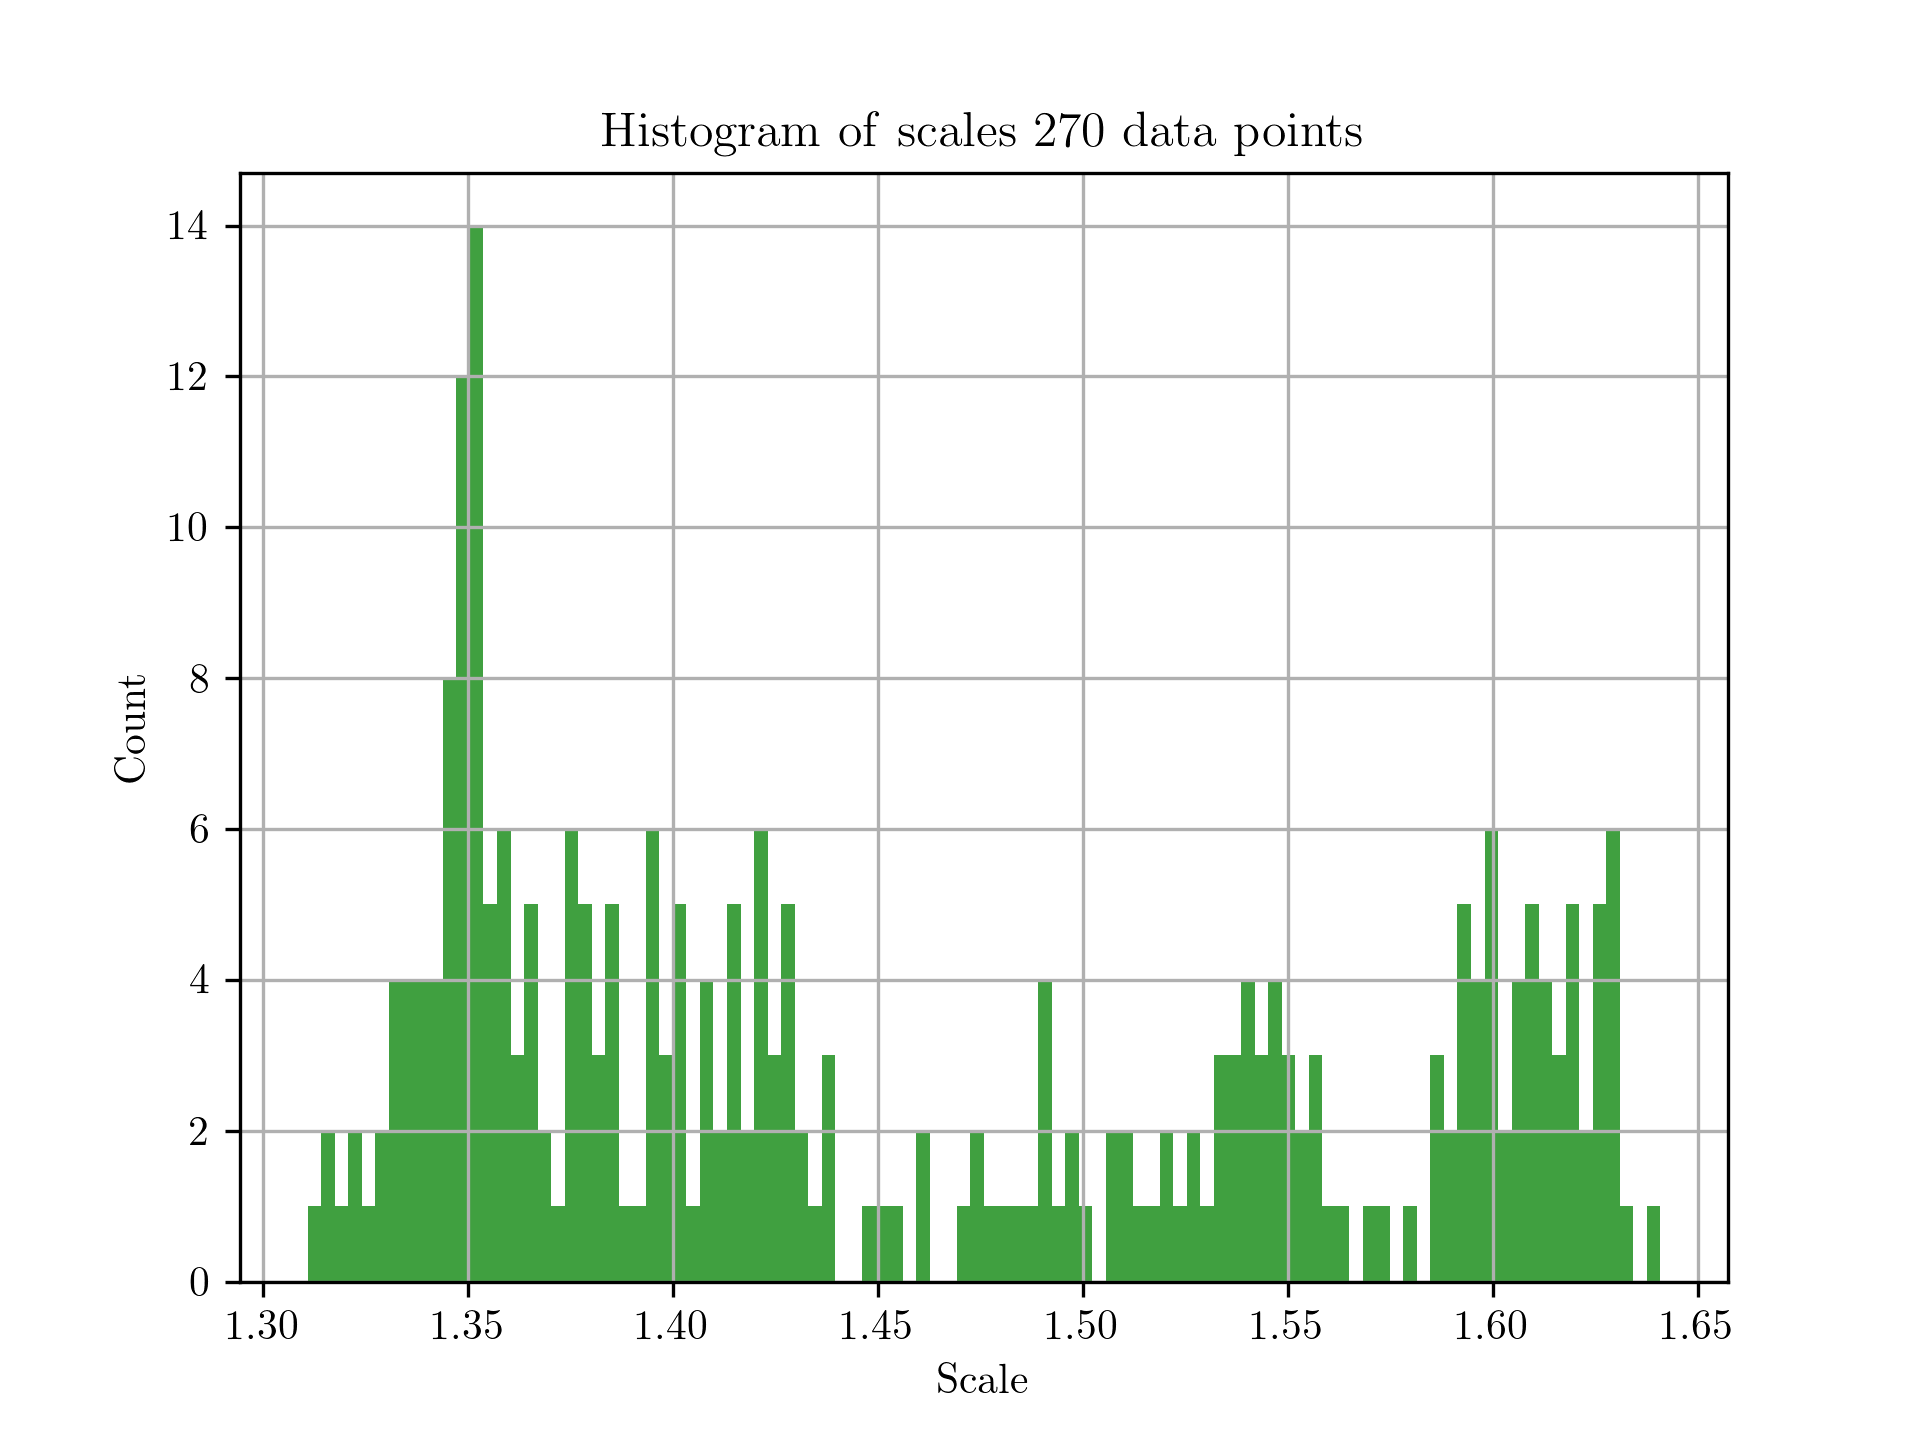
\includegraphics[width=0.9\linewidth]{stats_images4_rgb}
		\caption{images4}		
		\label{fig:stats_images4_rgb}
	\end{subfigure}
	\caption{Scale statistics for different image sets}
	\label{fig:scale_stats}
\end{figure}


\bibliographystyle{abbrv}
\bibliography{report_bib}

\end{document}

%%% Local Variables:
%%% mode: pdf
%%% TeX-master: t
%%% End:
